\chapter{Grundlagen}
\label{cha:grundlagen}

In diesem Kapitel sollen die Grundlagen vermittelt werden, die für das Verständnis der nachfolgenden Kapitel notwendig sind. Das folgende Bild zeigt die Struktur des Kapitels:

\begin{figure}[h]
\centering
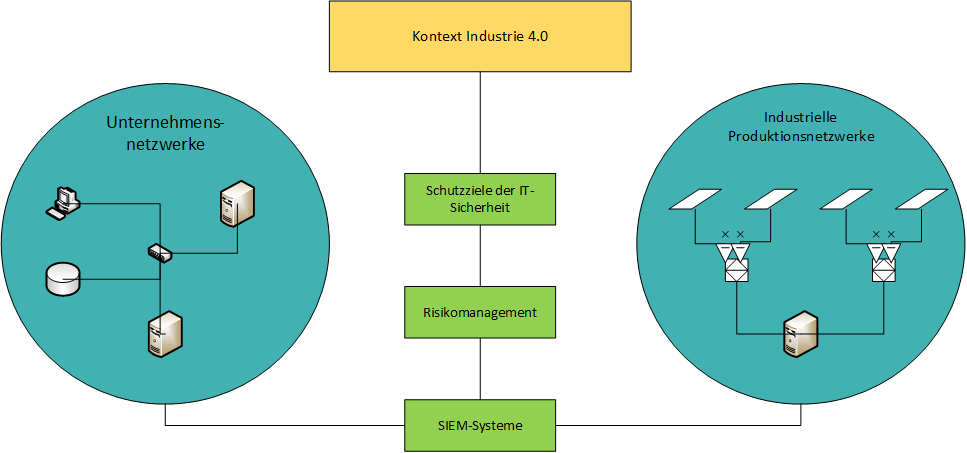
\includegraphics[width=175mm]{Zeichnungen/Grundlagenkapitel.png}
\caption{Aufbau des Grundlagenkapitels}
\label{fig:Aufbau des Grundlagenkapitels}
\end{figure}

Zunächst wird der Kontext der Industrie 4.0 beschrieben um ein Rahmenverständnis für den aktuellen Stand und die Idee der Vernetzung von Fertigungsanlagen zu vermitteln. Darauf folgend werden die grundlegenden Schutzziele der IT-Sicherheit definiert, welche die Basis für eine IT-Sicherheitsanalayse darstellen. Da eine Analyse aller relevanten Daten und Datenquellen auf Grund der limitierten Ressourcen eines SIEM-Systems nicht möglich ist, ist eine Risiko Management Strategie von fundamentaler Bedeutung. Aus diesem Grund werden die Grundlagen für Risiko Management in einer Sektion beschrieben. Aufbauend auf diesen Grundlagen erfolgt eine Beschreibung des SIEM-Systems- Konzepts, Komponenten und  Funktionalitäten. Dies soll ein Grundverständnis für die zu betrachtenden Datenmengen schaffen, die ein SIEM-System in die Analyse und Korrelation der Daten benötigt. Schlussendlich sind Grundkenntnisse zu den Elementen sowohl von Unternehmensnetzwerken als auch industriellen Automatisierungsnetzwerken notwendig, weshalb eine grobe Beschreibung dieser Elemente hinzugefügt wurde.

\section{Industrie 4.0 Konzept}
%Quelle: https://www.plattform-i40.de/I40/Navigation/DE/Industrie40/WasIndustrie40/was-ist-industrie-40.html
Das Konzept der Industrie 4.0 stellt einen Ansatz zur Steigerung der Flexibilität und Effektivität der Wertschöpfungsketten. Dazu sollen verschiedene industrielle Anlagen innerhalb einer Wertschöpfungskette über das Internet (WAN) miteinander verbunden werden und sogenannte \glqq Smart Factories\grqq geschaffen werden, die sich besser auf die Wünsche der Kunden einstellen können. Wichtige Punkte dieses Konzeptes sind die horizontale und vertikale Integration. Zum aktuellen Zeitpunkt sind Unternehmens- und Industrienetzwerke voneinander getrennt und/oder durch eine Sicherheitsschicht voneinander getrennt, sodass keine Kommunikation zwischen Industrienetzwerk und Internet durchgeführt werden kann. Das Konzept der vertikalen Integration soll diesen Zustand verändern, sodass Produktionsverwaltung per Web Interface erfolgen kann. Gleichzeitig soll über das Konzept der horizontalen Integration eine stärkere Verknüpfung und Kommunikation der Elemente auf den verschiedenen Netzwerkebenen erreicht werden\citep{Ind401}.


\subsection{Stand der IT-Sicherheit in industriellen Produktionsnetzwerken}
%Quelle: ICS Security - What is happening(?)
Industrielle Netzwerke wurden ursprünglich als isolierte Umgebungen entwickelt, sodass Sicherheitsmaßnahmen sich stärker auf den physischen Zugang zu den Anlagen als auf die Sicherung der IT Systeme konzentrierten \citep{6622964}. 

%Stuxnet
Durch das Auftreten von Stuxnet auf das iranische Atomprogramm und andere Angriffe auf industrielle Anlagen ist die Sicherung der Kommunikation und des virtuellen Zugriffes auf die Komponenten verstärkt als wichtiger Punkt anerkannt worden \citep{6622964}. 
%Kommunikationsprobleme
Da in industriellen Netzwerken unterschiedliche Kommunikationstechniken existieren, die teilweise keinerlei Schutzmechanismen z.B. für die Verifizierung der Kommunikationspartner oder der Integritätsprüfung der ausgetauschten Informationen bieten, sind industrielle Netzwerke nach aktuellem Stand potentiell anfällig für Angriffe. Dementsprechend ist die Sicherung dieser Netzwerke eine hohe Priorität, da bei einer Verbindung mit dem Internet ein potentieller Angriffsweg für Angreifer geschaffen wird, die bisher auf physischen Zugang oder das Einschleusen kompromitierter Speicher, wie z.B. USB Sticks, angewiesen sind \citep{6622964}. 

%IT-Security & industrial requirements
Neben den Schwachstellen der Kommunikationstechnologien ist die Sicherung bei gleichzeitiger Garantie der Verfügbarkeit eine weitere Herausforderung. 
%Update issue
So ist es nach aktuellem Stand nicht möglich, regelmäßige Sicherheitsupdates für SPSen aufzuspielen, da dies das Anhalten der Produktionsprozesse und damit signifikante Verzögerungen und finanzielle Verluste zur Folge hat. Darüber hinaus müssen Neuerungen an der SPS Firmware und/oder geladenen Programmen jeweils zertifiziert und überprüft werden um die Robustheit und Ausfallsicherheit zu garantieren. Dieser Zustand macht es schwierig gebräuchliche Sicherheitskonzepte aus Unternehmensnetzwerken in industriellen Netzwerken einzusetzen \citep{6622964}.

%Hier fehlt theoretisch im Detail: Authentifzierungsproblem Mitarbeiter, Darstellung der Sicherheitsmethoden, Probleme und Anforderungen ausführen

\subsection{Forschungsgebiete der IT-Sicherheit}
%Quelle: ICS Security - What is happening? (MTREsearch/20180424(IIoT Security ...))
Um die IT-Sicherheit der industriellen Netzwerk zu erhöhen und eine Möglichkeit zu schaffen, die Konzepte der Industrie 4.0 sicher umsetzen zu können, wird an verschiedenen Themenfeldern geforscht um Erkenntnisse zu gewinnen und Lösungen zu entwickeln. Quelle \citep{6622964} zeigt eine mögliche Klassifizierung dieser Felder. Die Autoren teilen die Forschung in die folgenden Themenfelder auf:
\begin{itemize}
\item Sichere Kontrolle
\item Erkennung von Eindringungsversuchen
\item Simulation und Modellierung
\item Kommunikations- und Infrastruktursicherheit
\end{itemize}

\subsubsection{Sichere Kontrolle (\glqq Secure Control\grqq  )} 
Unter diesem Begriff werden Forschungen zusammengefasst, welche sich mit dem Schutz von Informationen (d.h. Daten in der Speicherung und bei der Übertragung) befassen. Es gilt die Verfügbarkeit der Daten zu abzusichern, z.B. gegen Angriffe, die eine (langfristige) Störung als Ziel haben (Denial of Service (DoS)), sowie die Integrität und Vertraulichkeit der Informationen zu sichern (zur Vermeidung von fehlerhaften Ausführung und Täuschungen). Dabei spielt der Vertrauensgrad für die Korrektheit der übermittelten Daten (\glqq Veracity\grqq  ) eine wichtige Rolle. Dabei sollen nicht nur Daten des IT-Bereichs, sondern auch Prozessdaten einbezogen werden. Kernthemen sind etwa die sichere Identifizierung der Kommunikationsteilnehmer, Analyse von Entscheidungsmustern der Angreifer und damit verbundene Forschungen über die Robustheit bzw. die Anfälligkeit der Prozesses gegen Störungen.

\subsubsection{Erkennung von Eindringungsversuchen}
Wie in der klassischen IT-Sicherheit geht es bei diesem Gebiet darum herauszufinden in welcher Form industrielle Kontrollsysteme anfällig sind gegenüber Angreifern und die darauf basierende Entwicklung von Algorithmen und Maßnahmen um diese Angriffe zu erkennen und vorbeugende Maßnahmen zu treffen. Bereits entdecke Schwachstellen weisen u.a. unsichere Umsetzungen, aber auch Designfehler auf, die Angriffsmöglichkeiten eröffnen. Im Zuge dieses Themenfeldes haben sich Forscher auch u.a. mit dem Stuxnet-Programm beschäftigt, welches für die Manipulation des iranischen Atomprogramms verwendet wurde.

\subsubsection{Simulation und Modellierung}
Dieses Themenfeld beschäftigt sich hauptsächlich mit Fragen, die sich auf die Möglichkeit des Testens von IT-Sicherheitsmaßnahmen in industriellen Netzwerken beschäftigen. Die Grundproblematik teilt sich in zwei Elemente auf. Zum einen ist das Testen an realen Umgebungen sehr aufwendig, gefährlich und teuer, der Nachbau nicht öknomisch und aufwendig. Daher wird versucht mit sofware-basierten Frameworks zu arbeiten um die Arbeit eines automatisierten Fertigungssystems zu simulieren. Ein sehr wichtiger Punkt ist dabei die akkurate Simulation von physikalischen Prozessen und die fehlende Kompetenz/Fachwissen der Sicherheitsforscher in diesem Bereich. Andere Bereiche der Modellierung und Simulation beinhalten das (komplexe) Verhalten solcher Umgebungen und die Analyse von Kommunikationsmustern (Datenverkehr) innerhalb dieser Systeme.

\subsubsection{Kommunikations- und Infrastruktursicherheit}
Die Grundlage dieses Forschungsbereichs ist u.a. das Streben der Industrie nach einem einheitlichen Kommunikationsmedium in Form des Industrial Ethernets. Kernthemen sind dabei etwa die horizontale und vertikale Integration der Netzwerkteilnehmer und das Verpacken von Prozessdaten in Ethernet-Pakete und die damit verbundenen Herausforderungen der klassischen IT-Sicherheit. Hinzu kommt die wachsende Verzahnung und Abhängigkeiten der Teilsysteme und die Analyse von Risiken und Anforderungen für einen sicheren Betrieb. Forschungen dieses Bereichs richten sich damit u.a. auf Angriffsszenarien auf allen Hierarchieebenen des Netzwerkes von der Unternehmensleitebene bis zur Feldebene, etwa Angriffsszenarien mit dem Ziel der Beschädigung oder Zerstörung des Fertigungssystems.


\section{IT Security Schutzziele}
\label{cha:IT Security Schutzziele}

%Quelle: https://docstore.mik.ua/orelly/networking_2ndEd/ssh/ch03_01.htm
In der IT-Sicherheit werden alle Ziele bezeichnet, die für die Sicherung von Systemen und Kommunikation zwischen Systemen sichergestellt werden müssen. 
\todoForm{Mehr Kontext der Schutzziele einfügen}

Dabei werden als Grundlage die folgenden Schutzziele betrachtet:
\begin{itemize}
\item Integrität: Bei der Kommunikation zwischen Systemen und der Speicherung bzw. dem Abruf von Daten auf einem System ist es wichtig, dass darauf vertraut werden kann, dass diese Daten nicht ohne Authorisierung verändert wurden. Daher befasst sich dieses Schutzziel mit der Korrektheit von Daten bzw. der korrekten Funktion eines Systems. Bei der Sicherstellung dieses Zieles geht es also darum die Veränderung von übertragenen oder gesicherten Daten und Software sicherzustellen.
\item Vertraulichkeit: Innerhalb einer Infrastruktur oder auf einem System existieren verschiedene Arten von Daten, darunter auch sensible Daten,  die von nicht-authorisierten Personen missbraucht werden können. Daher ist es notwendig den Zugriff zu Daten zu limitieren und dadurch diese Daten vor unauthorisiertem Zugriff zu schützen. Aktivitäten dieser Art werden dem Schutzziel Vertraulichkeit zugeordnet
\item Verfügbarkeit: Diesem Schutzziel werden alle Aktivitäten zugeordnet, die den Betrieb von Systemen und die Erhaltung von Kommunikationswegen sicherstellen. Darunter fallen z.B. Maßnahmen, die den Zugriff von Kunden und/oder Mitarbeitern auf einen Webservice sicherstellen, auch im Falle eines Angriffes, der es zum Ziel hat die Erreichbarkeit des Services zu unterbinden.
\end{itemize}
\todoForm{Schutzziele: Beispiel für Schutzziele formulieren}
Neben diesen Schutzzielen existieren auch noch weitere Schutzziele wie z.B. Authentizität, Nichtabstreitbarkeit, Zurechenbarkeit und Privatsphäre.

\section{Risiko Management}
%Quelle 1: „IT Security Management“ (Mac, MTResearch/02082017/General/) - Kapitel 1.7 - 1.9 / Chapter 1

Risiko Management bezeichnet einen Bereich bzw. eine Sammlung von Aktivitäten, die der Abschätzung, Planung und Vermeidung von Risiken für ein Unternehmen bzw. eine Organisation dienen. Ein Risiko wird als Kombination aus der Eintrittswahrscheinlichkeit eines bestimmten Sicherheitsereignises und der damit verbundenen Konsequenzen definiert \citep{Partida2010}. Nach der ISO27001 
%Quelle 2: „IT-Sicherheitsmanagement nach der neuen ISO27001“ (Mac, MTResearch/02082017/General/)
definiert ein Sicherheitsereignis laut Quelle \citep{RM2} als eine Änderung eines Zustandes in der Informationsverarbeitung, welches mindestens theoretisch eine Auswirkung auf die Sicherheit haben kann. 
Die zentralen Begriffe für die Beschreibung eines Risikos sind \glqq Schwachstelle\grqq     und \glqq Bedrohung\grqq . Eine Schwachstelle wird im Kontext der Informationstechnologie als eine potentiell ausnutzbare Schwäche bzw. Fehler in einem Asset bezeichnet. Der Begriff \glqq Asset\grqq  beschreibt laut ISO27001 alles was für das Unternehmen bzw. die Organisation wertvoll ist, im Bezug auf Informationssysteme schließt dies u.a. Daten, Systeme, Anwendungen und Dienste (Services) ein. Unter einer Bedrohung wird widerum ein potentieller Auslöser für einen Sicherheitsvorfall verstanden, welcher Schaden am Unternehmen verursachen kann \citep{RM2}.

Daraus folgend wird das Risiko beschrieben durch die Wahrscheinlichkeit, dass eine Bedrohung konkrekt vorhanden ist und eine Schwachstelle ausnutzt.


Die Aktivitäten des Riskomanagement werden sowohl durch das NIST als auch durch den ISO27001 Standard in folgende Schritte zusammengefasst: Risikoabschätzung, Risikovermeidung, Risikoakzeptanz und Risikokommunikation.

Die Abschätzung potentieller Risiken ist der erste Schritt, der sich in verschiedene Unterpunkte gliedert. Dazu zählt zunächst die Identifikation potentieller Risiken und die Analyse der gefundenen Risiken. Von der Beschreibung eines Risikos, die aus der Analyse folgt, ist der Detailgrad sehr wichtig für die Präzision der Risiko Abschätzung \citep{RM2}. %Quelle 1: „IT Security Management“ (Mac, MTResearch/02082017/General/) - Kapitel 1.7 - 1.9 / Chapter 1
So kann etwa die Risikoabschätzung für die potentielle Ausnutzung einer Schwäche an einem Systems innerhalb des Unternehmensnetzwerkes präziser geschätzt werden, wenn der konkrete Zugriffsweg des Angreifers präzise beschrieben wird. Einen weiteren Unterpunkt der Risikoabschätzung stellt die Risikoevaluation ein, die die Bewertung und Beurteilung eines Risikos beinhaltet. Dies beinhaltet neben der konkreten Einschätzung einer Eintrittswahrscheinlichkeit auch die Erarbeitung potentieller Gegenmaßnahmen \citep{Partida2010}.

Der zweite Schritt umfasst die Risikovermeidung. Diese schließt die Priorisierung bestimmter Risiken sowie die Umsetzung und Pflege der Maßnahmen zur Vermeidung der priorisierten Risiken ein. 

Als dritter Schritt wird die Risikoakzeptanz genannt. In diesem Schritt werden die übrigen Risiken neu bewertet. An diesem Punkt können abhängig von der Entscheidung der Verantwortlichen weitere Gegenmaßnahmen eingeleitet oder aber auch Risiken als Restrisiko für das Unternehmen akzeptiert werden. 

Die resultierende Risiko Management Strategie wird im letzten Schritt mit betroffenen Vertragspartnern kommuniziert \citep{Partida2010}.

\section{Security Information and Event Management}
\label{cha:Security Information and Event Management}

\subsection{SIEM Konzept und Zweck}
\label{cha::SIEM Konzept und Zweck}
Im Umgang mit Security Information and Event Management (SIEM) Systemen werden oft die Begriffe „Information“, „Ereignis“ und „Daten“ verwendet. Um eine Grundlage für die Verwendung dieser Begriff in der vorliegenden Thesis zu geben, werden im folgenden diese Begriffe wie folgt definiert:
\begin{itemize}
\item Ereignis (Event): Unter einem Ereignis ist in diesem Zusammenhang das Auftreten von systemrelevanten Aktionen zu verstehen. Dabei kann zwischen Systemereignissen, z.B. das Laden eines Programmes, und Benutzerereignissen, z.B. Anschläge auf der Tastatur, unterschieden werden. 
\item Daten: Daten sind die Bausteine aus denen Ereignisse zusammengesetzt werden. Daten sind z.B. der Name des geladenen Programms oder der Wert einer Benutzereingabe.
\item Information: Eine Information ist in diesem Kontext die Interpretation verschiedener Ereignisse, die eine Aussage über den Zustand eines Systems ermöglicht.
\end{itemize}


Die IT Infrastruktur von Unternehmen umfasst eine große Menge an Elementen wie Server, Arbeitsstationen, Netzwerkgeräte, Sicherheitssysteme und mobile Endgeräte (z.B. Laptops und Mobilfunkgeräte). Um diese Infrastruktur zu schützen reicht es nicht diese hinter einem Schutzwall zu positionieren, es ist auch wichtig zu erfassen welche Aktionen von wem wie und von wo innerhalb des Netzwerkes ausgeführt werden. Daher ist es wichtig, dass es Informationsquellen gibt aus denen diese Informationen ausgelesen und bewertet werden können. In Unternehmens-netzwerken wird dies typischerweise von den Elementen selbst durchgeführt. So befinden sich z.B. auf einem Server mit den Betriebssystem Windows verschiedene Log-Dateien, die Informationen darüber speichern welcher Anwender sich zu welchem Zeitpunkt angemeldet hat, wie viele Versuche für die Eingabe des Passwortes verwendet werden und welche Prozesse von diesem Anwender ausgeführt wurden. 
Die Analyse dieser Log-Dateien kann fachkundigen Administratoren Aufschluss darüber geben welche Aktionen von dem Benutzer oder dem System durchgeführt wurden. Eine Herausforderung bei dieser Analyse ist die Bewältigung der schieren Menge an Informationen und das Filtern relevanter Ereignisse. Selbst eine geringe Anzahl an Systemen kann eine große Menge an Daten produzieren welche von einem Administratorenteam ohne Hilfe von Werkzeugen nicht zu bewältigen sind. Mit Hilfe technischer Werkzeuge können die Daten in Log-Dateien gefiltert werden. Die Suche nach sicherheitsrelevanten Informationen kann dabei automatisiert werden und Administratoren können über Anomalien im Verhalten der Systeme informiert werden. 

Allerdings bietet diese Vorgehensweise auch Nachteile. So ist die Definition der Regeln nach denen Werkzeuge Log-Dateien durchsuchen eine komplexe Aufgabe, denn diese Regeln müssen eng genug gefasst sein um die Anzahl der Sicherheitsmeldungen verwaltbar zu halten, aber auch weit genug um potentiell bedrohliche Situationen zu erkennen. Um eine bedrohliche Situation bewerten zu können müssen Administratoren nicht nur in der Lage sein die Meldungen des Werkzeuges zu verstehen, sondern diese auch im korrekten Kontext einordnen zu können. Diese Einordnung kann in komplexen Netzwerken sehr schwierig sein.

Um diese Einordnung zu vereinfachen und die Anzahl an Falschmeldungen („False Positives“) zu reduzieren ist es also notwendig nicht nur ein Element sondern verschiedene Elemente im Zusammenspiel zu betrachten und die Informationen dieser Netzwerkelemente zu verknüpfen, also einen Zusammenhang von Informationen von verschiedenen Elementen zu erfassen. Für die Unterstützung der Administratoren bei dieser Aufgabe wurden Security Information and Event Management (SIEM) Systeme entwickelt.


%Beschreibung des Security Information and Event Management (SIEM) Konzeptes
Ein SIEM System ist also ein System, welches Informationen aus verschiedenen Quellen extrahiert, die einzelnen Informationsquellen analysiert und die gewonnenen Informationen in einen Zusammenhang bringt. Durch Aggregation von ähnlichen Daten und Korrelation dieser Daten lassen sich einzelne Alarmmeldung in einen Zusammenhang setzen und neue Informationen über den Wert und den Kontext der Meldungen gewinnen. Dadurch ist es möglich den Zustand eines Netzwerkes und seiner Elemente über ein zentrales System zu überwachen und kritische Situationen zu erkennen, die durch das Betrachten einzelner Elemente nicht erkennbar sind. Das SIEM System bildet damit eine zentrale Verwaltungsschicht oberhalb der Netzwerkelemente.

Um diese Funktion auszuführen sind verschiedene Schritte notwendig. Die Aufgaben teilen sich dabei in zwei Bereiche auf: Security Information Management (SIM) und Security Event Management (SEM). SIM ist eine Unterkategorie des Log Management Feldes, das heißt es umfasst Erfassung, Extraktion, Transfer und Sicherung von sicherheitsrelevanten Informationen in Log-Dateien. SEM umfasst Funktionen für die Analyse und Verknüpfung von Ereignissen in Echtzeit.

Der erste Schritt ist die Extraktion der Daten von den Netzwerkelementen. Dies kann entweder durch Anbindung einer geeigneten Schnittstelle durchgeführt werden (z.B. Meldungen von Sicherheitssystemen wie einer Firewall oder einem Intrusion Detection System (IDS)) oder durch Extraktion der Informationen über Kollektoren in Form von Software Agents. Der zweite Schritt betrifft die Übertragung der extrahierten Informationen. Diese muss sicherstellen, dass die Informationen vollständig und unverändert übertragen werden, da veränderte Informationen die Informationsgrundlage verändern auf der das SIEM System seine Analyse durchführt. 

Da nicht jedes System gleich ist und auch Log-Dateien und -Formate sich deutlich unterscheiden können, müssen die vom SIEM empfangenen Informationen vorverarbeitet und in ein einheitliches Format umgewandelt werden. Dieser Schritt wird als „Normalisierung“ bezeichnet. Die normalisierten Daten können dann zentral gespeichert und für statistische Langzeitanalysen und statistische Verwertungen gespeichert werden. Dabei ist es wichtig darauf zu achten, dass die abgelegten Daten nicht verändert werden können und das Änderungen nachvollziehbar sind. Da die Datenmenge abhängig von der Größe und Komplexität sehr groß sein kann und die Ressourcen des SIEM Systems für die Analyse und Bewertung begrenzt sind, werden ähnliche Daten in einem Zwischenschritt zusammengefasst, sodass die zu analysierende Menge an Daten deutlich reduziert wird. Man spricht dabei von der Aggregation der Daten. Die Aggregation kann z.B. dadurch erfolgen, dass Ereignisse desselben Ursprungs und desselben Inhalts als eine Meldung zusammengefasst und mit einem Zähler versehen werden, der die Anzahl der Meldungen wiederspiegelt.
Im nächsten Schritt werden die aggregierten Daten dann durch ein Regelwerk analysiert. Dieses Regelwerk wird manchmal auch als „Rule Correlation Engine“ bezeichnet. Dabei werden verschiedene Meldungen mit Regeln abgeglichen. Wird eine Regel als erfüllt angesehen, wird eine Alarmmeldung an verantwortliche Administratoren ausgegeben, sodass weitere Maßnahmen ergriffen werden können.  Die Bewertung ob eine Regel erfüllt wurde hängt von der verwendeten Korrelationstechnik ab. So müssen z.B. eine Reihe von Bedingungen erfüllt werden, damit eine Regel als erfüllt angesehen wird. So könnte z.B. eine Regel beinhalten, dass ein Alarm ausgegeben wird, wenn mehrere nicht-erfolgreiche Anmeldungsversuche von einem inaktiven Account von einer nicht-registrierten IP-Adresse protokolliert wurden. Die Bildung solcher Regelwerke kann sehr komplex sein und durch verschiedene Techniken gebildet werden.


%Grenzen
In der Praxis werden SIEM Systeme u.a. in Security Operations Center (SOC) eingesetzt. Das SIEM hilft in diesem Kontext nicht nur den Administratoren für die Verwaltung, sondern ersetzt auch die Verwaltung und Analyse über verschiedenen UIs unterschiedlicher Sicherheitsprodukte (z.B. von Firewalls, IDSs, Anti-Virus Software). 
Hier zeigen sich neben den Vorteilen von SIEM Systemen auch aktuelle Grenzen. So kann ein SIEM nur auf der Informationsbasis operieren, die in der jeweiligen Umgebung zur Verfügung steht. So kann sich das Fehlen von Informationen zum Kontext der Meldungen auf die Auswertung auswirken, da fehlende Informationen zu ungenauen Analysen oder False Positives bzw. False Negatives (kritische Meldungen, die als harmlos klassifiziert werden) führen können. Eine andere Limitierung sind Abfragezeiten von gespeicherten Langzeitdaten für die Echtzeitanalyse durch die entweder die Analyse oder die Menge der Daten begrenzt wird. Auf der technischen Seite ergeben sich zudem Herausforderungen entlang der Funktionskette eines SIEM Systems bei der Datenextraktion aus proprietären Formaten, der effektiven und sicheren Speicherung der Daten sowie der Analyse und Erstellung von Korrelationsregeln in komplexen Systemen. 


\subsection{SIM \/ Log Management}
%Kontext
Security Information Management (SIM) bezeichnet die Verwaltung von Log-Dateien im SIEM Kontext und bildet damit eine Untermenge des Log Management. Sicherheitsrelevant sind in diesem Falle alle Log-Dateien, die Auskunft über den Zustand eines Systems oder einer Kommunikation zwischen Netzwerkelementen geben können. Dazu zählen sowohl Log-Dateien von Betriebssystemen und Programmen als auch von Netzwerkswitches und anderen Elementen, die den Datenverkehr zwischen Teilnehmern im Netzwerk aufzeichnen. Eine Log-Datei besteht aus Ereignissen, die Daten zu Aktionen (u.a. Zeitpunkt, ausführender Benutzer, ausführender Prozess (ID), …) enthalten. Diese Daten können interpretiert werden und liefern Informationen über den Zustand des Systems zum bestimmten Zeitpunkt.

%Definition
Log Management umfasst die Sammlung, Übertragung, Normalisierung, Zentralisierung und Aufbewahrung der Menge an Log-Dateien. In großen Unternehmen kann diese Menge mehrere hundert Gigabyte umfassen. Das Verwalten der Log-Dateien wird aus mehreren Gründen in Unternehmen als außerordentlich wichtig angesehen. Zum einen beinhalten Log-Dateien Informationen über den Zustand der Umgebung und können damit Rückschlüsse auf potentiell schädliche Aktionen zulassen, zum anderen können durch diese Informationen auch die Einhaltung von geltenden Richtlinien und Anforderungen gegenüber Kunden und Institutionen belegt werden. Daraus folgt, dass sichergestellt werden muss das die Informationen nicht nur korrekt aus den verschiedenen Quellen extrahiert werden können, sondern auch die Umwandlung und ggf. Veränderung der Daten dokumentiert werden muss um die Integrität der Informationen zu gewährleisten. Dies spielt u.a. für die Sicherheitsanalyse eine wichtige Rolle, da nur mit den richtigen Informationen die korrekten Rückschlüsse auf die Sicherheit der Umgebung geschlossen werden können. So lassen sich u.a. mit forensische Analysen rückwirkend Aktionsketten, die zu einer Richtlinienverletzung oder eines nicht-authorisierten Eindringens in das System geführt haben, rekonstruieren. Darüber lassen sich aus den Informationen Grundlagen für den Normalzustand eines Systems ablesen und entsprechende Regeln formulieren.
\todoForm{Log Management: Unterschied zwischen Log Management Systemen und SIEM Systemen herausstellen/formulieren}

Log-Dateien können aus fast jedem System gewonnen werden. Dazu zählen u.a. 
\begin{itemize}
\item Anti-Malware und Anti-Virus Systeme
\item Intrusion Detection Systems / Intrusion Prevention Systems
\item Remote Access Software
\item Web Proxieserver
\item Vulnerability Management Software 
\item Network Access Control (NAC) Server
\item Firewalls
\item Router
\end{itemize}

Eine interessantes Thema in diesem Zusammenhang ist die Frage welche Log-Dateien und Event-Daten sicherheitsrelevant sind. Moderne und komplexe IT-Umgebungen produzieren mehrere hundert Gigabyte an Event-Daten auf einer täglichen Basis. Daher ist die Definition sicherheitskritischer Elemente (Systeme, Kommunikationspfade, Applikationen, ...) eine wichtige Aufgabe.
Dazu können unter anderem diese Elemente gehören:
\begin{itemize}
\item Logs der Security Controls (z.B. Firewalls, Intrusion Detection System\/Intrusion Prevention System, Data Loss Protection)
\item Logs der Netzwerk Infrastruktur (z.B. Domain Name Service (DNS) Server, Dynamic Host Configuration Protocol (DHCP) Server, VPN Logs)
\item Informationen über die Infrastruktur aus anderen Quellen (z.B. Informationen zu Systembestand und Netzwerksegment eines Elements)
\item Informationen über das Unternehmen
\end{itemize}

\todoQuestion{Log Management: Log Management Architektur einfügen?}
\todoForm{Log Management: Beispiel für Log Management Architektur einfügen}

%Herausforderungen
Eine große Herausforderung des Log Management ist das Schaffen einer Balance zwischen limitierten, verfügbaren Ressourcen für das Verwalten der Log-Dateien und der Menge an zu verarbeitenden Log-Dateien pro Zeiteinheit. Dabei spielen nicht nur die potentiell große Menge an Dateien in einer komplexen Umgebung eine Rolle, sondern auch der Umgang mit Inkonsistenzen zwischen vergleichbaren Logs (etwa in Bezug auf den Zeitstempel), der Umwandlung aus verschiedenen Formaten und das Wachstum an Daten mit dem Hinzufügen von weiteren Systemen in die Umgebung.

\subsection{Kollektoren}
%Kontext
Die Extraktion, oder auch Sammlung, der Daten von den Elementen des Netzwerkes bildet die Grundlage auf der das SIEM System (und ein Log Management System) funktioniert. Die Daten werden von vielen verschiedenen Geräten extrahiert, die eine gewisse gemeinsame Grundmenge an Daten bieten, darüber hinaus aber auch weiteren Kontext abhängig von Applikation, Betriebssystem oder Gerät selbst. Daher muss eine Schnittstelle geschaffen werden, die diese proprietären Datenformate mit Hilfe eines Parsers auszulesen und zu einem einheitlichen Format umwandeln \citep{AV1}.
Dies ist die Aufgabe der Kollektoren. Eine weitere Aufgabe des Kollektors ist zudem die eines Filters für relevante Ereignisse. 

%Definition
Ein Kollektor ist demnach ein Service, oder auch Software Agent, der diese Aufgabe übernimmt. Dabei sind verschiedene Elemente zu betrachten, wie die verfügbaren Daten, Ressourcen der Datenquelle, Kommunikation zwischen Datenquelle, Kollektor und SIEM System sowie der Ansatz für einen bestimmten Gerätetyp. So stellt etwa das Protokoll, das für die Kommunikation mit der Datenquelle genutzt wird, eine Art Sprache dar, in der die Kommunikationspartner miteinander kommunizieren. Diese Kommunikationsform muss vorher vereinbart worden sein und dabei kann auf eine große Variation an Kommunikationsprotokollen zurückgegriffen werden. Der Kollektor für den entsprechenden Geräte-, Betriebssystem- oder Applikationstyp muss natürlich dieses Protokoll unterstützen. Alternativ dazu können Daten auch in weit verbreiteten Formaten wie etwa im „syslog“ Format abgelegt und durch den Kollektor oder eine Schnittstelle übermittelt werden.

%Kommunikationsmodelle
Bei dem Ansatz der Datensammlung kann bzgl. SIEM Kollektoren zwischen dem Agent-basierten und dem Agent-losen Ansatz unterschieden werden. Der Agent-basierte Ansatz wird durch die Installation der Kollektoren auf den jeweiligen Netzwerkelementen aufgebaut. Dadurch ergibt sich eine dezentrale Verarbeitung, die zum einen Ressourcen des SIEM System spart, zum anderen aber auch einen erhöhten Verwaltungsaufwand für Kollektoren auf den verschiedenen Elementen des Netzwerkes bedeutet. Der Agent-lose Ansatz hingegen nutzt Kollektoren als Schnittstelle, die vom zentralen SIEM System aus mit den Komponenten über Schnittstellen kommuniziert. Hier wird die Verwaltung der Kollektoren erleichtert, aber es muss auch die Netzwerklast berücksichtigt werden, die durch die Kommunikation zwischen den SIEM Kollektoren und den Datenquellen erzeugt wird. Zudem muss über die entsprechenden Schnittstellen sichergestellt werden, dass Daten nicht auf der Datenquelle selbst oder während der Übertragung verändert werden.

Orientiert an den Aussagen aus der Industrie wird mehr und mehr zum dezentralen Ansatz tendiert, da die Agenten zusätzliche Funktionalitäten bieten können sowie Herausforderungen im Bereich der Regelung von Remote-Administrations Rechten, Security Compliance, Ressourcenmanagement und der Speicherung von hoch privilegierten Zugriffsdaten zu verschiedenen Systemen auf einer zentralen Instanz. Allerdings ist der Einsatz von Agenten auf Elemente mit einem entsprechenden Betriebssystem beschränkt. Hardware-Elemente mit proprietären Betriebssystemen wie etwa Netzwerk-Geräte unterstützen den Agenten-basierten Ansatz nicht und müssen daher selbst die Informationen in einem für das SIEM verständlichen Format zu der SIEM Instanz schicken oder eine Schnittstelle für den administrativen Remote-Zugriff bieten.

\todoForm{Kollektoren: Füge Definition für "Parsing" hinzu}
\todoForm{Kollektoren: Zeige die Datenextraktion anhand eines Beispiels}
%Kollektor liest Events aus den Logdateien, bewertet die Events und schreibt diese in neue Logdateien, die zum zentralen Repository gesandt werden
%Kollektor fragt spezifische Events vom Zielsystem ab und wertet diese zentral aus

\subsubsection{Herausforderungen auf Basis von Log Dateien}
%Herausforderungen für Kollektoren
% Quelle: „Towards Structured Log Analysis“ (MTReseach/20180111)
Unabhängig von der Wahl des Ansatzes bestehen für die Analyse der Logs einige Herausforderungen, die auch oder im Speziellen Kollektoren betreffen. Da Logdateien pro System oder gar pro Anwendung in unterschiedlichen Formaten und mit unterschiedlichen Strukturen angelegt werden, muss ein Kollektor in der Lage sein, sowohl das Format, die Struktur als auch gängige Konstrukte zu erkennen und auszulesen. So muss ein Kollektor pro System, auf die systemspezifischen Schnittstellen und/oder Logdateien zugreifen können. Die Logdateien auf dem System können abhängig von der Systemart und/oder dem Betriebssystem bspw. als Textdatei, XML-Datei oder in einem binären Format abgelegt werden. Die Einträge innerhalb der Log-Dateien können einzeilig oder mehrzeilig gespeichert werden. Ein Kollektor muss in der Lage sein, diese Informationen zu erkennen und in den Lese- und Verarbeitungsprozess einfließen zu lassen \citep{6261962}. 

Neben diesen formalen Herausforderungen besteht zudem die Möglichkeit der Korruption von Logdateien sowie das Vorkommen von Inkonsistenzen. Ein Kollektor muss also in der Lage sein, den Lese- und Verarbeitungsprozess trotz fehlerhafter Einträge fortzuführen. Die Erkennung von Inkonsistenzen kann eine weitere Herausforderung im Bezug auf wiedersprüchliche Einträge, sofern dies Teil der Filterungsaufgabe des Kollektors ist. In diesem Bezug spielt natürlich auch die Performanz des Kollektors bei der Verarbeitung eine Rolle. So ist z.B. die Frage zu stellen, inwiefern bestimmte Logdateien einen sogenannten \glqq Performance Overhead\grqq  erzeugen basierend auf der Formatierung und der Menge des Inhalts \citep{6261962}.


\subsection{Event Verarbeitung}
\label{cha:Event Verarbeitung}
%Kontext
Durch die hohe Anzahl an Daten und Logquellen ist es notwendig relevante Einträge herauszufiltern und weiter zu verarbeiten, sodass die gewonnenen Informationen für die Überwachung und Analyse der Organisation verwendet werden können.

%http://raffy.ch/blog/2007/08/25/event-processing-normalization/
Die Ereignisdaten, die aus den Logs gewonnen werden, müssen daher zusammengefasst und auf Grund der Diversität der Logquellen vereinheitlicht werden. Aus diesem Grund können Logeinträge von den Kollektoren ausgelesen und sofern möglich die Daten in neue Logdateien mit einheitlichen Feldern transferiert werden. Im Kontext der SIEM Systeme gibt es verschiedene Begriffe und Ebenen für die Zusammenführung unterschiedlicher Datensätze zu einem einheitlichen Datensatz, im Bezug auf die Vereinheitlichung von Logeinträgen wird in diesem Fall der Begriff \glqq Normalisierung \grqq  verwendet. Dabei werden Logeinträge (Ereignisse) in verschiedene Kategorien unterteilt und die Daten in entsprechend strukturierten Datensätzen gespeichert \citep{EP1}.

%https://medium.com/@ateixei/get-over-siem-event-normalization-595fc36559b4
Diese kann, abhängig von der Menge an unterschiedlichen Logdateien und -quellen, auf Grund der notwendigen Vorarbeit für die Erarbeitung eines geeigneten Datenbank Schemas komplex oder sehr schwierig sein \citep{EP2}.

%Quelle: https://community.mcafee.com/people/andy777/blog/2016/02/21/siem-event-aggregation
Die zweite Aktivität im Bezug auf die Verarbeitung von Logeinträgen ist die Aggregation. Bei der Aggregation werden ähnliche Ereignisse, meist basierend auf bestimmten Feldern wie etwa Quell-IP, Ziel-IP und Event-ID, zu einem Ereignis zusammengefasst. Diese Methodik hilft dabei die Analyse der eingehenden Daten und kann damit die benötigte Menge an technischen und zeitlichen Ressourcen reduzieren. Auch kann sie ggf. bei der Vorverarbeitung helfen die Menge der zu übertragenden Informationen, und damit die Netzwerklast, deutlich reduzieren. Zu guter Letzt können durch die Reduzierung der Datenmenge diese Daten formatiert schneller und mit geringerem Speicherverbrauch gespeichert und abgerufen werden.
Die Verwendung von Aggregationsmethoden kann jedoch auch dazu führen, dass ggf. wichtige Daten nicht zur Verfügung stehen. Daher ist es in der Praxis wichtig, die Aggregationsmethodik bzw. -regeln abhängig von bestimmten Faktoren wie etwa der Häufigkeit oder Bedeutung im Bezug auf den Sicherheitskontext \citep{EP3}.

Diese Aufgaben können durch das zentrale System oder verteilte Agenten durchgeführt werden. 

\subsection{Security Event Management}
\label{cha:Security Event Management}

%Quelle: „SIEM as a Service - A survey“ (MTResearch/20182017)
Security Event Management befasst sich mit der Echtzeit-Analyse von normalisierten Events, der Korrelation dieser Events sowie der Benachrichtigung von Sicherheitsadministratoren und der Darstellung relevanter Informationen. Man kann in diesem Zusammenhang auch von kontext-bewusster Überwachung sprechen. %Quelle: „Building a Comprehensive IT Security Program“

Bei der Echtzeit-Analyse werden die extrahierten, normalisierten Events auf ihre Bedeutung untersucht. Dabei werden die Events einzeln für sich betrachtet und basierend auf den Daten(feldern) Informationen gewonnen. Diese Informationen werden bei der Korrelation der Events verwendet um einen Zusammenhang herzustellen. Dabei werden u.a. zusätzliche Informationen hinzugezogen, z.B. die Quelle der Informationen und Informationen zu der entsprechenden Quelle.
Dies ist notwendig um die Herstellung falscher Zusammenhänge zu minimieren. Die Herstellung der Korrelation basiert auf den verwendeten Techniken. So können Regelwerke auf verschiedene Art und Weisen hergestellt werden. Die Spannweite der Korrelationsregeln reicht dabei von simplen Wertevergleichen über Regeln mit verschiedenen Bedingungen hin zu der Erzeugung komplexer Szenarien durch Machine Learning und Big Data Ansätze. Wird eine Korrelationsregel erfüllt wird ein Alarm ausgegeben. Diese Alarme können abhängig von ihrer Priorität und Häufigkeit widerum durch Aggregationsregeln zusammengefasst werden.

%Quelle: The operational role of Security Information and Event Management Systems.pdf (MTResearch/20170814/Read)
Die durch die Korrelationsregeln ausgelösten Alarme helfen den Analysten in einer Organization kritische Situationen zu erkennen. Sie dienen dabei als Indikator für eine Kompromitierung (IoC, Indicator of Compromise). In größeren Organisationen sind die Analysten Teil eines \glqq Security Operation Centers\grqq  . In diesem Zentrum arbeiten Analysten mit verschiedenen Qualifikationen. So werden Indikatoren etwa zunächst von einem Analyst der Stufe 1 auf einen potentiell fälschlich ausgelösten Alarm (False Positive) untersucht und bei Feststellung eines Problems an Analysten der Stufe 2 weitergegeben. Diese Struktur dient zur effektiven Bewältigung der ausgelösten Alarme \citep{6924640}.


\subsection{Features \&  Gemeinsamkeiten von SIEM-System-Anbietern}
Für die allgemeine Betrachtung von SIEM Systemen kann es nützlich sein, die Gemeinsamkeiten und Unterschiede gebräuchlicher SIEM Anbieter zu kennen. Nach den Quellen \citep{SIEMVendors1,SIEMVendors3,SIEMVendors4}
%Quelle1: http://searchsecurity.techtarget.com/feature/Comparing-the-best-SIEM-systems-on-the-market
%Quelle2: http://infosecnirvana.com/siem-product-comparison-201/
%Quelle3: http://www.tomsitpro.com/articles/siem-solutions-guide,2-864-2.html
%Quelle4:  https://solutionsreview.com/security-information-event-management/7-siem-and-security-analytics-vendors-to-watch-in-2017/
gehören zu dieser (nicht vollständigen) Liste AlienVault, HP Enterprise, IBM, LogRythm, RSA, Solar Winds und Splunk. 

Die Produkte dieser Anbieter bieten jeweils ein Minimum an grundlegenden Funktionen eines SIEM Systems zusammen. Dazu zählt die Möglichkeit der Sammlung von Logs von vielen typischen Quellen, die Archivierung und Analyse der erhobenen Daten, sowie die Korrelation und Echtzeit-Überwachung der Quellen (d.h. Server, Netzwerkgeräte, Sicherheitslösungen, Anwendungen, etc.). Zusätzlich setzen die Produkte sogenannte \glqq Threat Intelligence Feeds\grqq  ein um (Kontext-)Informationen zu neuen Schwachstellen und/oder Bedrohungen zu erhalten. 


Die Unterschiede ergeben sich in der Architektur als auch in der Spezialisierung auf die Größe einer Organisation. 
Bzgl. der Architektur ergeben sich prinzipiell drei unterschiedliche Modelle: Cloud-basierte Lösungen, hardware-basierte Lösungen und anwendungsbasierte Lösungen. Cloud-basierte Lösungen bieten SIEM Funktionalitäten ausgelagert als einen Service an, der die Log-Quellen einer Organisation sammelt und analysiert. Hardware- und anwendungs-basierte Lösungen werden innerhalb der Infrastruktur der Organisation installiert und von dieser Organisation konfiguriert und gepflegt. Die Größe der Organisation kann dabei von sogenannten \glqq SMBs\grqq  (Small to Middle Sized Businesses) bis zu sehr großen und komplexen Infrastrukturen reichen.

Die Spezialisierungen der einzelnen Produkte können nach verschiedenen Kriterien festgelegt werden. Nach Studie der Quellen ergeben sich die folgenden Kategorien für Spezialisierungspunkte:
\begin{itemize}
\item Möglichkeiten der Erschließung von Logquellen - Dies kann entweder durch eine größere Menge an unterstützten Logquellen erfolgen oder durch eine flexiblere Anpassungsmöglichkeit (mit höherem administrativen Aufwand)(s. Splunk)
\item Möglichkeiten der Korrelation unter Einbeziehung der Logdaten sowie weiterer externer Quellen für die Integrierung von Kontextdaten wie etwa Threat Intelligence Feeds
\item Zusätzliche Fähigkeiten wie etwa \glqq Deep Packet Inspect\grqq  oder \glqq User Behavior Analytics\grqq
\item Möglichkeiten der Visualisierung des Status von Datenströmen und Netzwerken
\item Schwierigkeitsgrad der Installation und Einrichtung
\end{itemize}

Bei dieser Kategorisierung sein angemerkt, dass diese Liste keinesfalls vollständig ist oder sein kann. Nach den Einschätzungen der oben genannten Quellen muss für jede Organisation individuell geprüft werden, welche Fokuspunkte notwendig sind. Diese Kategorien geben lediglich grundlegende Elemente an.
Quelle \cite{SIEMVendors5}
% Quelle: http://searchsecurity.techtarget.com/feature/Comparing-the-best-SIEM-systems-on-the-market
etwa kategorisiert nach sieben grundlegenden Fragen: grundlegenden Unterstützung von Logquellen und -format, Möglichkeiten der zusätzlichen Protokollierung von zusätzlichen, relevanten Daten, die Nutzung und Qualität von Threat Intelligence Feeds, Möglichkeiten für forensische Analysen, zusätzliche Möglichkeiten für die Analyse und Examinierung von Daten, Qualität von automatischen Reaktionsmaßnahmen und Unterstützung für die Erfüllung von Industriestandards. 

\section{Infrastruktur Office}
Für den Vergleich zwischen Unternehmensnetzwerk und industriellem Netzwerk ist es notwendig beide Netzwerke zu kennen. Dieser Abschnitt stellt eine Fundament zur Verfügung auf dessen Basis die Analyse des Models eines Unternehmensnetzwerkes gestartet werden kann. Das Ziel ist es einen guten Überblick über die allgemeinen Elementtypen in solchen Netzwerkinfrastrukturen zu geben und ihre Kerncharakteristiken zu beschreiben und ihre Anordnung über Architekturtypen in den Kontext zu setzen. Neben den Netzwerkelementen als Quelle der Daten muss zudem die Kommunikation bzw. die verwendeten Kommunikationsschnittstellen in Form der Netzwerkprotokolle berücksichtigt werden, da die versendeten Pakete ebenfalls wichtige Daten enthalten um das Verhalten der System zu verstehen. Zuletzt soll noch eine grobe Übersicht über potentielle Angriffsszenarien bzw. -techniken gegeben werden. Die Kenntnis dieser Szenarien ermöglicht es später in der Analyse einen Bezug zu der Bedeutung der verfügbaren Daten des Netzwerkes herzustellen.

\subsection{Geräte}
Ein Unternehmensnetzwerk kann aus vielen verschiedenen Elementen bestehen. Dies beinhaltetet (verteilte) Anwendungen und Dienste, die auf der Basis von verschiedenenen, teils spezialisierten, Betriebssystemen installiert werden. Im Bezug auf physische Geräte können die Elemente jedoch in drei Basiskategorien unterteilt werden:
\begin{itemize}
\item Endgeräte (PCs, Laptop, Handy, ...)
\item Server
\item Netzwerkgeräte (Switches, Router, Firewalls, Sicherheitselemente (z.B. Intrusion Detection Systems))
\end{itemize}

Um Unternehmensprozesse durchzuführen werden verschiedene Server-Elemente benötigt. Ein Server ist ein zentrales Computerelement, welches mit mehreren anderen Elemente verbunden werden kann und entsprechenden Zugriff von diesen Elementen erlaubt. Zudem verfügen Server oft über leistungsfähigere Hardware und Speicherressourcen als ein Endgerät. Server werden benutzt um zentrale Applikationen bereitzustellen und zu verwalten. Dazu zählen neben Applikationen und (zugehörigen) Datenbanken auch Benutzerverwaltungssysteme und Sicherungscluster (Cluster := eine Menge an Servern, die durch eine zusätzliche Virtualisierungsschicht zu einem Element verknüpft werden). Zu den üblichen Serverarten zählen Webserver, Datenbankserver, Anwendungsserver, Proxyserver und Dateiablagesysteme, auf die über eine Netzwerkschnittstelle zugegriffen werden kann. 

Ein Webserver stellt über das Netzwerkprotokoll HTTP (Hypertext Transport Protocol) bzw. HTTPS erreichbare Dienste wie etwa Webseiten oder Webdienste zur Verfügung. Zu den typischerweise verwendeten Webservern zählen Microsofts IIS sowie Apache Webserver (meistens auf Basis eines Linux-basierten Servers wie etwa Ubuntu, CentOS oder RedHat). 
Ein Datenbankserver stellt den Zugriff auf eine strukturierte Menge von Daten in Form einer Datenbank über das Netzwerk zur Verfügung. Das verwendete Netzwerkprotokoll ist abhängig von dem installierten Datenbanktyp. Typische Datenbanken sind etwa Microsoft SQL Server, Oracle Database oder MySQL. 
Ein Anwendungsserver ist meist ein dedizierter Server für eine spezielle Anwendung, die einen Dienst für das interne Netzwerk bereitstellt. Beispiele sind etwa VPN-Server, Email-Server oder Sicherheitszugänge zu speziell geschützten Resourcen des Netzwerkes.
Dateiablagen (FTP Server) nutzen die File Transfer Protocol Schnittstelle um den Zugang zu auf dem Server gespeicherten Daten (z.B. Dokumente verschiedenen Typs) über das Netzwerk verfügbar zu machen. 
Proxyserver schließlich dienen als Zwischenpunkt zu einem anderen Netzwerk. Proxyserver werden z.B. benutzt um sonst vom WAN/Internet abgeschotteten Servern oder Endgeräten den kontrollieren Zugang zum Internet zu ermöglichen. 

Netzwerkgeräte dienen der Verbindung und/oder Überwachung der Kommunikation zwischen den einzelnen Netzwerkelementen. Diese lassen sich typischerweise in Router und Switche unterteilen. Router dienen der Verknüpfung mehrerer lokaler Netzwerke. Typischerweise existieren in Unternehmensnetzwerken eine Vielzahl an unterschiedlichen lokalen Netzwerken (auch Netzwerksegmente genannt), die es zu verbinden gilt. Daher kann im Rahmen dieser Netzwerken von zwei Routertypen gesprochen werden: \glqq Edge-Router\grqq  und \glqq Core-Router\grqq . Der Typ Edge-Router bezeichnet Router, die an den Grenzen des Unternehmensnetzwerkes zum WAN/Internet platziert sind, d.h. sie stellen die Verbindung zum Internet her. Core-Router widerum dienen dazu, die verschiedenen Netzwerksegmente innerhalb des Unternehmensnetzwerk miteinander zu verbinden. Diese Geräte existieren widerum, je nach Hierarchiestufe, in unterschiedlichen Fertigungen und sind angepasst für die jeweilige Aufgabe und Position im Netzwerk. 

Die Netzwerksegmente werden aus Sicherheitsgründen oft bestimmten Zonen zugewiesen (dazu später mehr im Abschnitt "Architekturtypen"). Die Verbindungen, die durch Core-Router hergestellt werden, werden typischerweise durch Firewalls abgesichert. Firewalls stellen eine Art vorkonfigurierten Filter dar, der abhängig von den konfigurierten Regeln und Parametern nur Datenverkehr mit bestimmten Netzwerkprotokollen aus und zu bestimmten Teilen des Netzwerkes zulassen.
Zusätzlich zu Firewalls werden außerdem Sicherheitselemente benötigt um den Datenverkehr zwischen den Netzwerkelementen zu überwachen. Diese Elemente werden Intrusion Detection Systems (IDS) bzw. Intrusion Prevention Systems (IPS) genannt. Ein IDS kann an einer bestimmten Stelle im Netzwerk platziert werden und ein Netzwerkpaket bzw. eine Sequenz von Netzwerkpaketen mitlesen und auf verdächtige Inhalte untersuchen. Für die Untersuchungsmethodik wird typischerweise eine Kombination aus der Suche nach bekannten Mustern im Datenverkehr als auch nach anomalen Datenpaketen oder -sequenzen verwendet.
Ein IPS ist prinzipiell ein Gegenstück zu einer Firewall. Die Aufgabe des IPS ist es den Datenverkehr zu analysieren und nach vorkonfigurieten Regeln Datenpakete von spezifizierten Netzwerkprotokollen aus spezifizierten Teilen des Netzwerkes zu blockieren.
Es existieren noch weitere potentielle Sicherheitselemente (wie etwa ein hardware-basierendes SIEM System), die jedoch in ihrer Grundfunktion auf Basis eines Server fungieren und daher hier nicht näher erläutert werden.

Endgeräte werden von Mitarbeitern und Gästen des Unternehmens verwendet als Zugangswerkzeug zum Unternehmensnetzwerk. Basierend auf den Richtlinien und Sicherheitsvorgaben sind diese Geräte deutlich eingeschränkt. Die Benutzer auf den Endgeräten werden üblicherweise in eine Domäne eingebunden um eine zentrale Benutzerverwaltung zu ermöglichen. Endgeräte können sowohl stationär als Arbeitsstation als auch mobil in Form von Laptops, Tablets oder Mobiltelefonen existieren. 

\todoForm{Sicherheitsanforderungen (Zweck und grobe Beschreibung) formulieren}

\subsection{Architekturen \&  Anforderungen}
Unter \glqq Unternehmensarchitekturen\grqq  bzw. dem Design dieser Architekturen versteht man eine Sammlung an Architekturen aus verschiedenen Perspektiven. Diese definieren die verschiedenen Sichten und Schichten die ein Unternehmen definieren. Im speziellen wird der Begriff Unternehmensarchitektur definiert als eine zusammenhängendes Ganzes von Privilegien, Methoden und Modellen, die genutzt werden im Design und der Umsetzung von organisatorischen Unternehmensstrukturen, Unternehmensprozessen, Informationssystemen und -Infrastrukturen \citep{Lankhorst2017}. %Quelle: https://link.springer.com/content/pdf/10.1007%2F978-3-662-53933-0_1.pdf
Im Kontext der Betrachtung von Informationsquellen für SIEM Systemen wird hier nur die Infrastruktur der  technischen, sicherheitsbezogenen Architektur betrachtet. Das Ziel ist es eine grobe Übersicht zu vermitteln um einen Kontext für die Realtionen der Netzwerkelemente zu vermitteln.


Während die Architekturdetails, oder genauer definiert die Infrastrukturelemente, abhängig von anderen Modellen und Perspektiven gestaltet werden, lassen sich folgende grundlegende Kommunikations-Bereiche definieren: Extranet (Zugang zum globalen Netzwerk), demilitarisierte Zone (Zugangsbereich zum Unternehmen) und Intranet (internes Netzwerk des Unternehmens), ggf. mit weiteren Unterteilungen \cite{Stingley2015}. %Quelle:https://www.sans.org/reading-room/whitepapers/bestprac/infrastructure-security-architecture-effective-security-monitoring-36512

\todoImage{Bild für typische Enterprise Technical Architecture Infrastructure einfügen}
%Quelle: Exploring the Enterprise Network Infrastructure.pdf (MTResearch/20170928/Read)
Zunächst besteht eine Verbindung zum Internet (Extranet), diese wird durch gesicherte Gateways ermöglicht. Damit allerdings keine direkte Verbindung von diesen Gateways in das interne Netzwerk gewährt wird, wird eine zusätzliche Netzwerkzone zwischen das Gateway und das interne Netzwerk geschaltet. Diese Zone wird de-militarisierte Zone (DMZ) genannt. Innerhalb der DMZ werden Server angebunden, die aus dem Internet erreichbar sein sollen. Dies umfasst u.a. Webserver, die einen oder mehrere Webservices beherbergen oder Sprungserver (z.B. für eine VPN-Verbindung). Diese Server werden im Bezug auf ihre Kommunikationsfähigkeit limitiert, sodass keine Netzwerkverbindung von diesen Servern in das interne Netzwerk hergestellt werden kann, nur in umgekehrter Richtung ist die Herstellung einer Verbindung möglich. Das interne Netzwerk widerum kann in viele verschiedene weitere Netzwerkzonen und Domänen unterteilt sein. Diese Segmentierung dient der Strukturierung des Netzwerkes und eröffnet zusätzlich die Möglichkeit weitere Sicherheitsschichten in die Umgebung einfließen zu lassen. Das interne Netzwerk beherbergt Endgeräte von Mitarbeitern, Server mit Firmendaten, Datenbankserver und Datensicherungscluster. Alle Elemente in einer solchen Umgebung sowie die Kommunikation zwischen diesen Elementen können von verschiedenen Sicherheitssystemen überwacht werden. 

\subsection{Kommunikation}
In Unternehmensnetzwerken kommunizieren die Elemente auf Basis der Ethernet-Technologie und dem Internet Protocol (IP). Der zugehörige TCP/IP Stack bestimmt die grundlagen der Kommunikation durch die Zuweisung einer eindeutigen IP Adresse. Die Zuweisung dieser IP Adresse kann fest zugeordnet werden (z.B. für Server), manuell erfolgen oder automatisch über das Dynamic Host Configuration Protocol (DHCP) erfolgen, welches einem neuen Netzwerkelemente automatisch eine freie IP Adresse aus einem Adressenpool zuweist. Die meisten Elemente in einem Netzwerk werden einer sogenannten Domäne zugeordnet. Eine Domäne ist eine Zusammenstellung verschiedener Netzwerkelemente, die eine zentrale Benutzerverwaltung für die zugehörigen Elemente erlaubt. 
%Quelle: https://www.appliedtrust.com/resources/infrastructure/understanding-dns-essential-knowledge-for-all-it-professionals
Zu einem der wichtigsten Netzwerkdienste zählt der \glqq Domain Name Service\grqq  (DNS). Dieser Netzwerkdienst erlaubt es den Namen einer Domäne einer oder mehreren IP-Adressen zuzuordnen und übernimmt die Beantwortung von Anfragen zur Namensauflösung. Die Namensauflösung wandelt einen Domänennamen in eine zugehörige IP-Adresse um, die von dem anfragenden Gerät genutzt werden kann um eine Verbindung herzustellen. Dies ermöglicht menschlichen Benutzern die Möglichkeit eine bestimmte Domäne (z.B. \glqq google.de\grqq ) über ihren Namen anzufragen anstatt über das Wissen um die korrekte IP-Adresse (die sich ggf. ändern kann) verfügen zu müssen. Die Ausführung der Anfrage und Empfang der Antwort wird von einem lokal installierten \glqq DNS-Resolver\grqq  übernommen. Der DNS ist ein hierarchischer Verzeichnisdienst, das bedeutet, dass die Administration und Namensauflösung über ein hierarchisches Netz bestehend aus Namensservern durchgeführt wird. Der Namensraum des Internets wird dabei in einem hierarchischen Baum zunächst in sogenannte \glqq Top-Level Domains\grqq  (z.B. \glqq de\grqq ) unterteilt, die widerum in weitere Subdomänen unterteilt werden. Der von rechts nach links zusammengesetzt Pfad ergibt den Namen der Domäne. Dieser hierarchische Aufbau ermöglicht den strukturierten Aufbau der Namen und eine umgekehrt hierarchische Abfragemöglichkeit für die Namensauflösung. Diese Konzept kann nicht nur im Internet, sondern auch lokal innerhalb eines Unternehmensnetzwerkes verwendet werden \citep{DNS1}.
Basierend auf der IP-Adresse kann eine verbindungsorientierte Kommunikation per Transmission Control Protocol (TCP) oder eine verbindungslose Kommunikation per User Datagram Protocol (UDP) erfolgen.  Ist es eine Priorität, dass eine Nachricht vollständig und in richtiger Reihenfolge übertragen wird, wird z.B. TCP verwendet. Auf weiteren zusätzlichen Schichten können weitere Funktionalität wie etwa eine kryptografische Verschlüsselung erfolgen. 
%Quelle: https://www.elektronik-kompendium.de/sites/kom/0301201.htm
Die verschiedenen Schichten sind u.a. im OSI-7-Schichtenmodel festgehalten.
Das OSI-Modell bietet eine herstellunabhängige Grundlage für das Design von Kommunikationsprotokollen und Computernetzwerken. Das OSI-Modell unterteilt die Kommunikation in sieben Schichten:
\begin{itemize}
\item Schicht 7: Anmeldung - Funktionen und Anwendung
\item Schicht 6: Darstellung - Umwandlung von Daten in ein systemunabhängiges Format
\item Schicht 5: Kommunikation - Steuerung des Datenaustausches (Sessions)
\item Schicht 4: Transport - Zuordnung von Datenpaketen zu einer Anwendung
\item Schicht 3: Vermittlung - Routing
\item Schicht 2: Sicherung - Segmentierung der Pakete 
\item Schicht 1: Bitübertragung - Umwandlung für die physikalische Übertragung
\end{itemize}

Jede Schicht fügt den vorherigen Schichten neue Elemente hinzu um die Kommunikation um zusätzliche Funktionalitäten und Eigenschaften zu erweitern \citep{OSI1}. 

\todoForm{Enterprise Kommunikation - VPN \& Remote Access beschreiben}


\subsection{Bekannte Angriffsvektoren}
%Kontext
Für das Risiko Management wie auch für die Implementierung von Verteidigungsmaßnahmen ist es notwendig die gebräuchlichen Angriffsvektoren zu kennen, die ein potentieller Angreifer nutzen kann um unberechtigterweise auf Komponenten in einem Unternehmensnetzwerk zuzugreifen. 

%Definition
%Quelle: https://www.techopedia.com/definition/15793/attack-vector
Ein Angriffsvektor ist eine Technik, durch die ein Angreifer ein Netzwerk oder Netzwerkelemente angreifen oder ausnutzen kann. Angriffsvektoren helfen dabei Schwachstellen der angegriffenen Komponente, inklusive dem menschlichen Benutzern, auszunutzen. Eine Schwachstelle kann ein programmierter Fehler in einer Anwendung sein, ein Fehler in der Prozesskette einer Anwendung, Schnittstelle oder eines Netzwerkprotokolles oder eine Lücke in der Absicherung der Komponente \citep{AttackVector1}. 

Da es viele verschiedene Komponenten in einem Unternehmensnetzwerk gibt in vielen verschiedenen Versionen und mit vielen verschiedenen Abhängigkeiten, Kommunikationsprozederen und Anwendungsarten, ist es nicht möglich sich hundertprozentig for Angriffen zu schützen. Jedoch ist es möglich durch Kenntnis von bekannten Angriffsvektoren Schwachstellen zu schließen und somit das Risiko eines erfolgreichen Angriffes zu verringern und diesen zu erschweren.

Für Unternehmensnetzwerke lassen sich Angriffsvektoren grob in die folgenden Kategorien unterteilen \citep{Campbell2016}
\begin{itemize}
\item \glqq Malware\grqq 
\item \glqq Denial-of-Service\grqq
\item \glqq Angriffsvektoren auf Webinhalte \grqq
\end{itemize}


%Vektoren 
%Quelle: https://link.springer.com/content/pdf/10.1007%2F978-1-4842-1685-9_10.pdf
\subsubsection{Malware}
Malware, auch Schadsoftware, ist der Überbegriff für Programme, die auf einem Computersystem mit bösartiger Absicht ausgeführt werden. Eine Malware kann etwa dazu benutzt werden um über den infizierten Host auf Informationen und andere Komponenten des Netzwerkes zuzugreifen, die Resourcen des Hosts in Form von Rechenleistung, Netzwerkbandbreite, o.ä. zu nutzen oder den Host zu kontrollieren.
Eine populäre Methode um Malware auf einem Ziel auszuführen ist die Versendung als Anhang von gefälschten E-Mail, etwa in der Form von Spam-Emails oder  Phishing-Emails (personalisierte E-Mails für den entsprechenden Benutzer) oder auch Spear-Phishing (speziell angepasste E-Mails nach Hintergrundrecherchen der Zielperson). Der Angreifer versucht in diesem Falle den Benutzer dazu zu bringen etwa einen Link zu einer gefälschten Webseite anzuklicken, über die der Schadcode im Hintergrund auf den Computer des Ziels heruntergeladen wird, oder einen modifizierten Anhang zu öffnen, durch den der Schadcode auf dem Computer installiert wird. Gängige Malwaretypen sind trojanische Pferde, Computerviren, Computerwürmer, \glqq Rootkits\grqq , logische Bomben  und Spionageprogramme\citep{Campbell2016}.

Die Unterscheidung dieser Typen ist wichtig, da die Funktionalität und Operation der verschiedenen Typen Auskunft über potentielle Indikatoren geben kann. Aus diesem Grund werden die verschiedenen Typen im Folgenden kurz beschrieben. 
Ein Computervirus  ist ein Programm, welches im Programmcode eines modifzierten Programmes oder einer modifizierten Datei versteckt ist. Wie der biologische Virus benötigt dieser Malware-Typ einen Host, also anderes Programm oder einen Prozess, um sich weiter zu verbreiten. Ein Computerwurm hingegen ist eine unabhängige Anwendung und kann sich unabhängig von seinem Host der Ressourcen des Hosts bedienen um sich weiterzuverbreiten. Sowohl Computerviren als auch Computerwürmer werden genutzt um weitere Computer im Einflussbereich des infizierten Hosts zu infizieren und den Einfluss des Angreifers auszuweiten. 
Ein Rootkit wird verwendet oft in diesem Zusammenhang verwendet um seine eigene Ausführung und die Ausführung anderer Malware zu verbergen, etwa durch das Verbergen der Prozess im Windows Task Manager oder durch Blockierung des Benutzerzugriffes auf sein Quellenverzeichnis. Dafür wird das Rootkit oft als Folgeschritt der Infizierung eines Hosts von einer Quelle heruntergeladen und mit administrativen Privilegien installiert um Zugriff auf die Betriebssystemkomponente zu erlangen.
Eine weitere Malware-Art ist das sogenannte \glqq trojanische Pferd\grqq . Diese Art von Malware ermöglichen die Ausführung von Kommandos auf dem infizierten Host ohne das Wissen des Benutzers und können unabhängig von den Operationen des Hosts ausgeführt werden. Trojanische Pferde ermöglich u.a. die Öffnung von Hintertüren, die dem Angreifer den Zugriff auf das kompromitierte System ermöglichen. Diese Technik wird oft für die Erstellung oder Erweiterung von Botnetzen verwendet. Botnetze bestehen aus einer Sammlung kompromitierter Systeme, die von einem \glqq Command\& Control-Server\grqq  gesteuert werden können. Dieser Server (Botmaster) ermöglicht die Versendung von Befehlen an die kompromitierten Systeme (Bots) zur Ausführung dieser Befehle auf den Systemen.
Logische Bomben sind eine Malware-Art, die auf ein System heruntergeladen, deren Ausführung jedoch verzögert wird bis eine vordefinierte Bedingung bzw. eine Sammlung von Bedingungen erfüllt werden. Dies kann von einem bestimmten Zeitpunkt (Datum) bis zu komplexen Abhängigkeiten von Versionen installierter Software, Patches oder anderer Systemvariablen reichen.
Unter \glqq Spyware\grqq  versteht man eine Malware, die Informationen des kompromitierten Systems an den Angreifer übermittelt. Dies können z.B. Tastatureingaben (Key Logger), Screenshots (Screen grabber) oder  auch Videostreams vom aktuellen Bildschirm sein\citep{Campbell2016}.

\subsubsection{Denial-of-Service}
Neben dem Ziel Informationen zu stehlen oder System zu kontrollieren kann ein Angreifer auch das Ziel haben die Erreichbarkeit (s. Schutzziele) eines Webservers oder eines Webdienstes zu unterbinden, etwa um finanziellen Schaden oder rufschädigende Auswirkungen zu erzielen. Dieser Angriffsvektor wird als \glqq Denial-of-Service \grqq  bezeichnet. Die Unterbindung der Erreichbarkeit wird durch das Aufbrauchen einer notwendigen Resource erreicht, etwa Bandbreite, Anzahl der maximalen Verbindungen zum Server oder Rechenleistung. Um dieses Ziel zu erreichen wird üblicherweise eine hohe Anzahl an Systemen benötigt, die gemeinsam den Angriff ausführen. Aus diesem Grund werden z.B. die beschriebenen Botnetze verwendet um parallel eine große Anzahl an Anfragen an einen Server zu senden um die Bandbreite auszulasten. Durch die verteilte Natur dieses Angriffes werden diese Angriffe als \glqq Distributed Denial-of-Service\grqq  Angriffe bezeichnet\citep{Campbell2016}.

\subsubsection{Angriffsvektoren auf Webinhalte}
Bei diesem Angriffsvektor werden Schwachstellen von Webinhalten ausgenutzt, die den Zugang zu Informationen oder das Ausführen von Schadcode auf dem unterliegenden Webserver ermöglichen. Dieser Vektor lässt sich weiter unterteilen in \glqq Active Content\grqq  Angriffe und \glqq Content Injection\grqq  Angriffe. 
Als Active Content werden Webinhalte bezeichnet, die Funktionalitäten zu Webseiten hinzufügen. Dazu zählen etwa JavaScript, PHP, Adobe Flask, Perl, HTML5 und Java. Oft bringen diese Inhalte vollständige Programmierumgebungen mit sich, die eigene Schwachstellen und ausnutzbare Fehler enthalten können. So kann etwa durch das Ausnutzen einer Schwachstelle JavaScript Code in eine Webseite integriert werden, der ausgeführt wird, wenn ein anderer Benutzer diese Webseite aufruft um bspw. Malware auf den Computer des Benutzers herunterzuladen. 
Der Vektor Content Injection wird meistens durch fehlende Überprüfungsroutinen einer Webanwendung geöffnet. Durch das Einfügen von spezifischen Eingaben, die von den gewollten Eingabewerten abweichen wird etwa das Abrufen von Benutzerdaten einer Datenbank über ein Login-Feld oder die Möglichkeit des Stehlens von Cookies der Benutzersitzung über \glqq Cross-Site Scripting\grqq  (XSS) ermöglicht, welches die Möglichkeit der Impersonifizierung des Benutzers gegenüber der Webanwendung eröffnet\citep{Campbell2016}.

\section{Infrastruktur industrielle Produktionsnetzwerke}

\todoForm{Kontext der industriellen Infrastruktur einfügen}

\subsection{Architektur \&  Anforderungen}
%Prozesskontrolle
Die Architektur eines industriellen Netzwerkes ist darauf ausgelegt, einen Fertigungsprozess zu kontrollieren. Dementsprechend existiert eine hierarchische Struktur, welche die Kontrolle des Prozesses von der Aufgabenannahme bis hin zur Kontrolle der einzelnen Schritte durch SPSen, Aktoren und Sensoren. Zu diesem Zweck wird auf die Disziplin der Prozesskontrolle zurückgegriffen. Die Prozesskontrolle ist eine Ingenieursdisziplin, die sich auf Architekturen, Mechanismen und Algorithmen für die Aufrechterhaltung der Funktionalität eines Prozesses beschäftigt. Allgemein spricht man bei Elementen innerhalb der Prozesskontrolle von industriellen Kontrollsystemen. Diese Kontrollsysteme können in verschiedenen Architekturen abgebildet werden.

\subsubsection{Die Automatisierungspyramide}
%Quelle: 20180212/Industrial Networks/Grundlagen der Automatisierung
Um das Zusammenspiel und die Anordnung / Strukturierung der Komponenten in einem industriellen Netzwerkes zu verstehen, ist es sinnvoll die grundlegenden Konzepte hinter einer solchen Architektur zu beleuchten. 
Die Grundlage bildet die industrielle Automatisierung, durch die sich ein industrieller Fertigungsprozess abbilden lässt.
Ein automatisierter Fertigungsprozess ist ein Prozess, der ohne das Eingreifen von Menschen ablaufen kann und bei dem ein Material oder ein Produkt mit Energie und Informationen umgewandelt wird \citep{Linke2017}. 
Die industrielle Automatisierung durchzieht verschiedene Hierarchieebenen, die unterschiedliche Aufgaben erfüllen. Für die Darstellung dieser Ebenen kann auf die Automatisierungspyramide verwiesen werden.
\todoImage{Einfügen eines Bildes der Automatisierungspyramide}
Es wird zwischen den folgenden Hierarchieebenen unterschieden:
\begin{itemize}
\item Unternehmensleitebene
\item Betriebsleitebene
\item Produktionsleitebene
\item Prozessleitebene (mit weiteren Unterteilungen)
\item Feldebene
\end{itemize}

In der Unternhemensleitebene werden Prozesse durchgeführt, die die Ausrichtung des Unternehmens bestimmen. Dazu werden u.a. sogenannte Enterprise Resource Planning (ERP) Systeme (z.B. von SAP) für die Verwaltung der zur Verfügung stehenden Resourcen sowie für die Verwaltung der kaufmännischen Prozesse eingesetzt.
Die Betriebsleitebene hat die Aufgabe die eingehenden Aufträge zu verwalten und fristgerecht durchzuführen, inklusive der Produktionsplanung und der Verwaltung und Überwachung der täglichen Betriebsprozesse \citep{Linke2017}. In dieser Ebene werden MES-Systeme für die Produktionssteuerung und Kontrolle der Fertigung in Echtzeit eingesetzt \cite{MES1}. %Quelle: http://www.softselect.de/business-software-glossar/mes-manufacturing-execution-system
Die kurzfristigere Planung des Einsatzes bestimmter Maschinen oder Anlagen ist Teil der darunterliegenden Produktionsleitebene. In dieser Ebene werden sogenannte Supervisory Control and Data Acquisition (SCADA) Systeme eingesetzt. \todoResearch{SCADA-Systeme, siehe Handbuch Quelle}
Die Prozessleitebene strukturiert die verschiedenen Fertigungszellen des Produktionsprozesses. Abhängig von der Größe der Anlage, kann sie in mehrere Unterebenen unterteilt werden, die widerum hierarchisch die Anlage, Gruppen von Fertigungszellen und einzelne Fertigungszellen (Zellebene) abbilden. Innerhalb dieser Fertigungszellen wird ein bestimmter Bearbeitungsprozess durchgeführt, der durch verschiedene Bearbeitungsmaschinen durchgeführt wird. Die Bearbeitungsmaschinen werden durch speicherprogrammierbare Steuerungen (SPS) kontrolliert, die ihrerseits Daten aus der Feldebene und übergeordneten Systemen erhalten.
Zu der Feldebene werden Aktoren, Sensoren und Anzeigegeräte gezählt, d.h. diese Ebene umfasst die Erfassung und Weiterleitung von (Mess-)Daten sowie die Ausführung von veränderten Stelldaten, die als Reaktion auf die ausgewerteten Informationen der Messdaten veranlasst werden\citep{Linke2017}.

%Quelle?
%Eine mögliche Form ist die Supervisory Control and Data Acquisition (SCADA) Architektur. In dieser Architektur existieren prinzipiell vier verschiedene Ebenen (von Level 4 (Verwaltung) zu Level 0 (Sensoren und Aktoren):
%\begin{itemize}
%\item Level 4 repräsentiert die Schnittstelle zum Unternehmensnetzwerk. Systeme auf dieser Ebene sind für die Produktionsplanung verantwortlich.
%\item Level 3 repräsenteirt die Produktionskontrolle über die Anlage. Systeme auf dieser Ebenen kontrollieren den Produktionsprozess indirekt durch die Überwachung von Zielen und Produkten.
%\item Level 2 beinhaltet weitere Systeme für die Beaufsichtigung wie z.B. den Leitstand. Die Elemente werden genutzt um Aktionen auf Level 1 und Level 0 zu kntrollieren. Human Machine Interfaces (HMI) gehören zu diesen Elementen und stellen eine grafische Benutzeroberfläche für Mitarbeiter zur Verfügung. Außerdem beinhaltet dieses Level das verteilte Kontrollsystem.
%\item Level 1 ist die Ebene mit direkter Kontrolle auf die Prozessschritte über die angeschlossenen SPSen.
%\item Level 0 beinhaltet Sensoren und Aktoren, die für die Kontrolle und Anpassung der Prozessschritte verwendet werden
%\end{itemize}

\subsubsection{Prozessleittechnik und Architekturanforderungen}
%Quelle: 20180212/Industrial Networks/Grundlagen der Automatisierung
Auf der Grundlage der oben beschriebenen Ebenen, ihre Funktion und ihre Aufgaben wird im folgenden der Begriff der Prozessleittechnik und die damit in Verbindung stehenden Anforderungen an die Komponenten der Architektur beleuchtet. 
Die Prozessleittechnik ist eine Unterkategorie der Produktionsleittechnik. Sie betrachtet Aspekte der Mess-, Steuer- und Regelungstechnik sowie die systematische Ordnung von Produktionsprozessen, die Informations- und Kommunikationstechnik sowie die Konzeption für das Erstellung und Betreiben von Leitsystemen. Damit dient die Prozessleittechnik als Schnittstelle zwischen der technischen Umsetzung des Prozesses und der Beobachtung/Bedienung des Prozesses durch den Menschen. Sie bildet das Zusammenspiel zwischen Prozessleitebene und Feldebene ab. 
Die Grundfunktion der Prozessleittechnik ist die Erfassung, Übertragung, Verarbeitung und Ausgabe von Prozessdaten für die Steuerung und Überwachung des Produktionsprozesses. Dafür müssen abhängig von den Informationen, die aus den verarbeiteten Daten gewonnen werden, Entscheidungen innerhalb eines bestimmten Zeitraumes getroffen werden um Fehlfunktionen zu vermeiden. Dies wirkt sich allerdings auf die Qualität der getroffenen Entscheidung aus. Aus diesem Grund wird die Entscheidungsfindung hierarchisch auf verschiedene Teilsysteme (Unterebenen) aufgeteilt, die eine geringe Menge an Daten verarbeiten müssen. Durch diese hierarchische Struktur wird die Informationsdichte zu den oberen Ebenen hin höher, die Anforderungen bzgl. Reaktionsschnelligkeit und Zuverlässigkeit/Verfügbarkeit können jedoch im Vergleich zu den unteren Ebenen mit weniger Priorität betrachtet werden. 
Neben der Verfügbarkeit und Zuverlässigkeit ist auch die Robustheit gegenüber Fehlern eine Anforderung. Auch diese Anforderung ist durch die autarken Teilsysteme in der grundlegenden Architektur eines Fertigungssystems verankert.
Im Bezug auf Soft- und Hardwareanforderungen sind die Anforderungen ebenfalls abhängig von der Hierarchieebene. In der Feld- und Prozessleitebene ist die Anzahl der Teilnehmer an der Kommunikation ist geringer und die zu übertragenden Datenmengen vergleichsweise klein, dafür ist es wichtig, dass Anweisungen sehr schnell (in Echtzeit) gesendet und verarbeitet werden können. Dazu werden zusätzlich standardisierte Softwarebausteine verwendet um die Zuverlässigkeit des Programmablaufs zu maximieren. 
In den oberen Ebenen wie etwa der Betriebsleitebene werden andere Anforderungen wie in einem Unternehmensnetzwerk priorisiert\citep{Linke2017}. 

\subsection{Geräte}
In industriellen Netzwerken werden verschiedene Komponenten und Technologien auf den verschiedenen Ebenen der Prozesskontrollstruktur eingesetzt. Zu den Hauptkomponenten zählen:
\begin{itemize}
\item Speicherprogrammierbare Steuerung (SPS)
\item Human-Machine Interface (HMI)
\item OPC Server
\item Sensor \& Aktuator
\item Weitere Server und Arbeitsstationen der Büroebenen
\end{itemize}

\subsubsection{Speicherprogrammierbare Steuerungen}
%Definition SPS
%Quelle: 20180302/Industrial Networks/SPS-Quelle
Eine speicherprogrammierbare Steuerung (SPS) ist ein Gerät, welches Maschinen und Anlagen steuern oder regeln kann. Für die Steuerung als auch für die Regelung einer Maschine wird ein vordefiniertes Programm verwendet, welches auf der vorhanden Firmware ausgeführt wird. Die Firmware beinhaltet die verwendbaren Operanden und Programmbausteine, die für die Programmierung genutzt werden können. Für die Programmierung selbst werden von vielen SPSen standardisierte Bausteine der Norm IEC 61131-3 unterstützt \citep{Hoenle2017}.
%Paperquellen
Das auf die SPS geladenen Programm verarbeitet Informationen, welche von den Eingangsmodulen empfangen werden. An die Eingangsmodule sind üblicherweise ein bestimmter Sensortyp angeschlossen, welcher Informationen über einen bestimmten Aspekt des Prozessschrittes liefert. Basierend auf der Implementierung des Programms, dies kann z.B. eine logische Sequenz, eine Zeitschaltung oder eine arithmetische Operation sein, wird durch diese Informationen ggf. über ein Ausgangsmodul ein Aktor (z.B. ein Motor) aktiviert, der ein Element des Prozessschrittes kontrolliert und Änderungen anstößt oder durchführt. Ein Programm kann mehrere Operanden kombinieren und in Zusammenhang setzen, inklusive Input, Output, Arguments, Counter, Timer und Function Blocks.
%Quelle: 20180302/Industrial Networks/SPS-Quelle
Eine modulare SPS besteht aus mehreren Basiskomponenten, zu der noch weitere Module optional hinzugefügt werden können. Das Basisset umfasst mindestens einen sogenannten Baugruppenträger, d.h. einen Kasten in dem die Module platziert werden können, eine Stromversorgung, eine Baugruppe, welche die CPU und den Speicher enthält sowie digitale und analoge Ein- und Ausgänge für spezifische Elemente der Feldebene. 
Dazu können noch weitere Module wie etwa ein Kommunikationsprozessor (Communication Processor (CP)) 
für die Anbindung der SPS an ein Netzwerk, weitere Kommunikationsmodule sowie Zähler-, Positionier- oder Regelungsmodule \citep{Hoenle2017}. 
%Handbook
%Diese Flexibilität mit der direkten Anbindungsmöglichkeit an Elemente der Feldebene und die Fähigkeit Hochleistungslasten zu tragen zeichnet die SPS als Automatisierungsmotor in der industriellen Fertigung aus.

\subsubsection{Sensoren und Aktoren}
%Sensoren und Aktoren
%Quelle: Handbook
Auf der Feldebene werden neben speicherprogrammierbaren Steuerungen Sensoren und Aktoren eingesetzt. 
Ein Sensor ist ein Element, welches Änderungen einer physikalischen Gegebenheit in seiner Umgebung registriert und in ein elektronisches Signal umwandelt. Sensoren sind ein wichtiges Element, da Daten aus dem Produktionsprozess mit hoher Zuverlässigkeit und zeitnah an die kontrollierende SPS bzw. die Prozesskontrolle übermittelt werden müssen \citep{Jeong2009}. Sensoren sind üblicherweise als Teil des Schaltkreises eines Sensorgerätes. Abhängig von der Art des Sensors reagiert das Sensorelement auf eine bestimmte physikalische Veränderung. Sensoren unterscheiden sich daher in der Art der wahrgenommenen  Veränderung, zu denen in der Automatisierungsindustrie u.a. die folgenden zählen:
\begin{itemize}
\item Änderung des Widerstands
\item Änderung der Kapazität
\item Änderung der Induktivität
\item Elektromagnetische Induktion
\item Thermoelektrischer Effekt
\item Sonar
\item Optische Veränderung
\item Hall
\end{itemize}

Durch die technologische Entwicklung stehen heutzutage auch sogenannte Mikrosensoren zur Verfügung. Mikrosensoren, oder auch \glqq Smart Sensors\grqq , integrieren signalverarbeitende Schaltkreise, Analog-Digital-Wandler, programmierbaren Speicher und Mikroprozessoren in ein Sensorgerät. Zudem ist es auch möglich über die Integration einer Antenne eine kabellose Verbindung zu ermöglichen und Sensoren in kabellosen Sensornetzwerken (Wireless Sensor Networks (WSN)) zu strukturieren\citep{Jeong2009}.

Aktoren ermöglichen es per SPS auf die prozessnahen Maschinen des Produktionsprozesses einzuwirken und den Prozess zu kontrollieren. Aktoren verwenden u.a. Federmechanismen, hydraulische und/oder pneumatische Geräte, Magnetismus oder Termalenergie. Analog zu den Sensoren ist es möglich Aktoren mit zusätzlichen Elemente auszustatten um u.a. die Kommunikationsmöglichkeiten zu erweitern\citep{Jeong2009}.

\subsubsection{Human Machine Interface (HMI)}
%Quelle: https://ipc2u.de/catalog/automatisierungstechnik/hmi/
Ein Human Machine Interface, oder auch Mensch Maschinen Schnittstelle (MMS), ist die Bedienungsschnittstelle zwischen Mensch und Maschine. Sie dienen daher als Element für die Steuerung und Beobachtung der Prozesse durch einen Menschen. In der industriellen Fertigung werden HMIs in Form von Panelen, Stand-alone PCs oder auch Thin Clients (d.h. mit der Prozesskontrolle vernetzte Monitore) eingesetzt \citep{HMI1}. 
%Quelle:  http://w3.siemens.com/mcms/human-machine-interface/de/bediengeraete/basic-hmi/Seiten/Default.aspx
Die Anwendung einer bestimmten Hardwareform für die Benutzerschnittstelle wird dabei durch den speziellen Zweck als auch durch die Einsatzumgebung bestimmt. Die verschiedenen Typen unterscheiden sich dabei u.a. durch die Kommunikationsmodule, Größe und Art des Displays, Performance und angebotenen Zusatzmodulen\citep{HMI2}.
%Quelle: https://ipc2u.de/catalog/automatisierungstechnik/hmi/
HMIs sind oft auf einen speziellen Zweck spezialisiert, der durch den Einsatz und die konfiguration spezialisierter Softwarekomponenten umgesetzt wird\citep{HMI1}. 
%Sekundärquelle: http://www.indusoft.com/blog/2013/04/19/unterschied-zwischen-scada-und-hmi/

\subsubsection{Server und industrielle PCs}
%-------------------
%Definition
Die bereits im Unterkapitel \glqq Infrastruktur Office\grqq  definierten Server-Komponenten finden auch verschiedene Einsatzmöglichkeiten in industriellen Produktionsnetzwerken. Abhängig von der betrachteten Hierarchieebene werden diese Server für verschiedene Zwecke eingesetzt. Während Server in den oberen Hierarchieebenen Aufgaben des Büroumfeldes wie etwa die Funktion als Datenbankserver übernehmen, werden Server der Produktionsleitebene und speziell der Prozessleitebene für Kontroll- und Überwachungsfunktionen des Produktionsnetzes eingesetzt. 


%SCADA
%Wikipedia und die unten genannten Quellen
Eine Anwendungsmöglichkeit ist es den Server als SCADA-Server oder -System zu nutzen. SCADA steht für Supervisory Control and Data Acquisition und beschreibt ein wahlweise zentrales oder dezentrales Softwaresystem, welches Informationen der prozessnahen Komponenten (PNK) sammelt, die Informationen zu Analyse- und Überwachungszwecken verarbeitet und steuernd in den Prozess eingreifen kann. Dabei werden die PNKs als sogenannte Datenpunkte betrachtet, die auf Basis von bestimmten E/A-Werten und mathematischer Berechnungen bestimmt werden. 
%Quelle: https://www.itwissen.info/SCADA-supervisory-control-and-data-acquisition-SCADA-Protokoll.html
Zu den Betriebssystemen, die die Ausführung eines SCADA-Systems erlauben zählen u.a. DOS-basierte, Windows NT-basierte, Unix-basierte und Linux-basierte Betriebssysteme. Abhängig von der Größe des SCADA-Systems können mehrere tausende bis hunderttausende E/A-Kanäle umfassen\citep{SCADA2}. 
%Quelle: http://www.indusoft.com/blog/2013/04/19/unterschied-zwischen-scada-und-hmi/
In Richtung der oberen Hierarchieebenen kann ein SCADA-System u.a. mit ERP \& MES Systemen kommunizieren\citep{SCADA3}.

%Quelle: https://www.itwissen.info/SCADA-supervisory-control-and-data-acquisition-SCADA-Protokoll.html
Ein SCADA-Server kommuniziert auf verschiedenen Ebenen. Zu Bedien- und Beobachtungszwecken kann ein SCADA-Client mit einem SCADA-Daten-Server kommunizieren per TCP/IP-Schnittstelle. Die Daten-Server kommunizieren je nach Kommunikationspartner entweder über ein bestimmtes Feldbussystem (z.B. Profibus) mit PNKs oder untereinander über die Ethernet-Schnittstelle. Für die Kommunikation zwischen verschiedenen SCADA-Systemen kann das SCADA-Protokoll \glqq Sinaut\grqq  verwendet werden\citep{SCADA2}.


%OPC
%Quelle: Wikipedia & weitere
Der Zugriff von SCADA- und Prozessleitsystemen auf Elemente der Feldebene kann sowohl direkt oder über Prozesskontrollserver erfolgen. Ein Prozesskontrollserver ist ein Server mit zusätzlichen E/A-Schnittstellen, die für die Anbindung herstellerspezifische PNKs genutzt werden können. Um die herstellerspezifischen Datensätze in einem einheitlichen Format an die höheren Hierarchieebenen weiterleiten zu können, bedient man sich der OPC-Schnittstelle. Diese Schnittstelle erlaubt es mithilfe eines spezifischen OPC-Treibers die Datensätze in OPC-Objekte umzuwandeln und OPC-Funktionen zu unterstützen. Die OPC-Schnittstelle dient also zu der Sammlung von Daten aus einem Netzwerk von Sensoren, Aktoren und SPSen unterschiedlicher Hersteller. 
Abhängig von der OPC-Spezifizierung basiert OPC auf der DCOM-Schnittstelle von Microsoft und erfordert somit, dass der Server ein Windows-Betriebssystem verwendet. Diese Spezifizierung, das klassische OPC, umfasst Spezifizierungen für die Übertragung von Echtzeitdaten, Alarmen und Events, Zugriff auf historische Datensätze und die direkte Kommunikation zwischen OPC-Servern.
Der neuere OPC-Standard wird OPC-UA (Unified Architecture) genannt. Das Ziel dieses Standards ist es u.a. einen Standard unabhängig von DCOM und einem bestimmten Betriebssystemtyp für die zyklisch gesteuerte Kommunikation mit PNK-Netzwerken zu setzen.


%Industrielle PCs
%Quelle: Wikipediaartikel
In industriellen Produktionsnetzen werden auch PCs in Anlagen verwendet. Diese unterscheiden sich im Vergleich zu herkömmlichen Büro-PCs durch erhöhte Hardware- und Softwareanforderungen. Zu den Hardwareanforderungen zählen u.a. eine gewisse Robustheit gegenüber Einflüssen der Umgebung wie extreme Temperaturen, Schmutz, Feuchtigkeit oder elektromagnetische Felder und Vibrationen, aber auch eine gute Abschirmung des Gehäuses und der Anschlüsse (in Umgebungen, die empfindlich auf Störgrößen dieser Art reagieren). 
Unabhängig von der Umgebung müssen diese Computer jedoch vorallem ein hohes Maß an Zuverlässigkeit bieten und eine schnelle und einfache Wartung ermöglichen (z.B. die Möglichkeiten eine Festplatte innerhalb von Sekunden auszutauschen). Dies erfordert auch, dass die gleiche Hardware über einen langen Zeitraum betrieben werden kann, da Änderungen der Hardware zu Fehlern bzw. zur Unbrauchbarkeit von gesicherten Speicherabbildern führen können. 

Zu den wichtigen Softwareanforderungen gehören vorallem die zuverlässige, fehlerfreie Ausführung sowie die Verarbeitung von Daten in Echtzeit. Zu diesem Zweck wird etwa die Hauptplatine eines PCs durch ein speziell angepasste Platine mit mehr Steckplätzen für Busschnittstellen verwendet.

%Weitere Systeme
%Quelle: Handbook, Grundlagen der Automatisierung
Ein Fertigungssystem umfasst noch weitere Elemente wie etwa Systeme, die die Produktion von der Produktionsleitebene steuern (Manufacturing Execution System (MES)) oder die Überwachung und Verwaltung auf dieser Ebene ermöglichen über einen Leitstand, der alle Informationen des Fertigungsprozess zentral sammelt und darstellt. Auf der Feldebene existieren zudem noch speziellere Maschinen, etwa für die Qualitätssicherung des Produktes, den Transport des zu verarbeitenden Materials oder für das Austauschen verwendeter Werkzeuge. Da jedoch eine tiefere Beschreibung dieser Elemente für die Kategorisierung der verfügbaren Informationsmenge nicht erforderlich sind, sei an dieser Stelle jediglich darauf verwiesen, dass diese Elemente in diesen Netzwerken existieren \citep{Hoenle2017}.

\subsection{Kommunikationstechnologien}
%Kontext
In industriellen Netzwerken herrschen abhängig von der Hierarchieebene unterschiedliche Anforderungen an die Kommunikationswege zwischen den Komponenten. Während in den oberen Hierarchieebenen die Anforderungen der Unternehmensnetzwerke gelten, sind für die Kommunikation in den Bereichen der Prozessleitebene und Feldebene die Anforderungen der Echtzeitfähigkeit und der deterministischen Eigenschaft des Kommunikationssystems oder -protokolls zu erfüllen. Unter der Echtzeitfähigkeit versteht man die Fähigkeit eines Kommunikationssystems Daten innerhalb weniger Millisekunden oder sogar unterhalb einer Millisekunde zu übertragen. Dies ermöglicht eine schnelle Erkennung von Veränderungen innerhalb des physikalischen Prozesses und schnelle Reaktionen auf diese Veränderungen. Die notwendige Übertragungsgeschwindigkeit ist abhängig von der notwendigen Reaktionszeit. Die Anforderung des Determinismus beschreibt die \textit{Garantie} das Daten innerhalb eines bestimmten Zeitraumes übertragen werden. Diese Anforderung ergibt sich daraus, dass die Steuerungen garantiert mit den aktuellen Daten versorgt werden müssen um Reaktionszeiten einzuhalten und die Sicherheit der Anlage und der Mitarbeiter zu gewährleisten. Durch die technologischen Eigenschaften des Ethernetstandards ist dieser Determinismus nicht gegeben.

Die verwendeten Kommunikationssysteme in diesen Ebenen verwenden entweder Kommunikationsprotokolle, die den vorhandenen Ethernetstandard um diese Fähigkeiten oder verwenden andere Datenbustechnologien. Für die Kommunikation innerhalb der Prozessleitebene zwischen den OPC-Servern und hierarchisch höher liegenden Systemen wie etwa dem SCADA-System oder dem Leitstand wird der Ethernetstandard durch Kommunikationsprotokolle erweitert. Diese werden unter dem Begriff \glqq Industrial Ethernet\grqq Protokolle zusammengefasst. Für die Kommunikation mit den Steuerungen innerhalb der Feldebene werden historisch bedingt Feldbusse eingesetzt. Allerdings finden auch hier vermehrt Industrial Ethernet Protokolle Einzug. Die Basis für die Verwendung der Feldbusse ist die taktbezogene Arbeitsweise der speicherprogrammierbaren Steuerungen. Für die Steuerung der Sensoren und Aktoren werden widerum andere Busse wie etwa der AS-I-Bus oder der HART-Bus verwendet. Netzwerke, die aus Sensoren und Aktoren bestehen für die bessere und redundante Überwachung des Prozesses werden als Aktor-Sensor-Netzwerk bezeichnet.

%Erklärung der grundlagen eines Datenbuses? (A-)synchronität, Simplex & Duplex, 

%Feldbus
\subsubsection{Feldbus}
%Erster Satz sollte sein: Ein Feldbus ist ein...
\glqq Unter Feldbus versteht man ein Bussystem, dass in rauer Umgebung (Feld) eingesetzt wird. Neben besonderen Anforderungen an die mechanische Ausführung sind insbesondere auch Anforderungen an die Robustheit (Störempfindlichkeit) des Datenprotokolls. \grqq \citep{Gutekunst2017} %Quelle: Buchkapitel 
%--- Erklärung 1
Ein Bussystem ist ein Kommunikationssystem, bei dem mehrere Kommunikationsteilnehmer die gleiche Datenleitung (Datenbus) verwenden. Um die Kommunikation möglich zu machen, darf nur ein Teilnehmer pro Zeiteinheit als Sender agieren, während die anderen Teilnehmer den Datenbus abhören. Man spricht in diesem Zusammenhang auch von einer Punkt-zu-Gruppe Kommunikation\citep{Gutekunst2017}. %Quelle Buchkapitel
Für die Freigabe bzw. das Recht eines Teilnehmers Daten zu senden existieren verschiedene Modelle, deren Ausprägung abhängig sind von der verwendeten Topologie und der benötigten Funktionalität. Eine Form ist das sogenannte Master-Slave-Prinzip. Bei diesem Prinzip fragt ein autorisierter Teilnehmer (Master) Informationen der anderen Teilnehmer (Slaves) an und erteilt für den Empfang der Daten die temporäre Sendeerlaubnis. Dieses Prinzip wird in vielen Feldbussystemenen verwendet wie etwa PROFIBUS\citep{Gutekunst2017}. 
Für die Feldebene gilt, dass die Zuverlässigkeit der Kommunikation und die Verfügbarkeit der Daten garantiert werden muss. Ein entscheidender Faktor ist dabei die Behandlung von Kollisionen, welche auftreten wenn mehrere Teilnehmer gleichzeitig auf dem Datenbus senden. Zu diesem Zweck wird entweder CSMA/CD (Kollisionseerkennung) und CSMA/CA (Kollisionsvermeidung) verwendet. Bei der Kollisionserkennung stoppen alle Teilnehmer das Senden von Daten und der Teilnehmer mit der Sendeerlaubnis wiederholt das Senden der Nachricht. Durch diese Wiederholung kann es zu unterschiedlich großen Zeitfenstern kommen in denen eine Nachricht gesendet wird. Dieser Zustand kann zu Problemen in einer taktgesteuerten Umgebung wie der Feldebene führen wenn eine Nachricht innerhalb eines bestimmten Zeitfensters gesendet werden muss, d.h. die Kommunikation muss \glqq deterministisch\grqq  sein. Zu diesem Zweck wird die Methode der Kollisionsvermeidung verwendet, bei der Datentelegramme höherer Priorität Datentelegramme niedrigerer Priorität bei den Empfängern überschreiben sodass die Daten nicht erneut gesendet werden müssen. In Kombination mit dem Master-Slave-Prinzip, durch das quasi eine temporäre Punkt-zu-Punkt Verbindung zwischen Master und Slave hergestellt wird, kann eine deterministische Kommunikation implementiert werden\citep{Gutekunst2017}.
%--- 
Feldbusnetzwerke sind standardisierte, aber auch proprietäre Netzwerke. In den Standards IEC 61158 und IEC 61784 existieren zehn verschiedene Konzepte. Sieben dieser Konzepte stellen eine eigene Protokoll Suite zur Verfügung, die anderen drei Konzepte basieren auf Ethernet Funktionalität. Beispiele für Protokolle sind etwa PROFIBUS oder DeviceNet.


%Industrial Ethernet
\subsubsection{Industrial Ethernet}
%Warum Ethernet im industriellen Bereich? (Kontext)
Zusätzlich zu der Feldbustechnologie existieren in industriellen Netzwerken auch abgewandelte Formen des Ethernet Standards. Im Folgenden wird diese Abwandlungskategorie als \glqq Echtzeit-Ethernet\grqq  bezeichnet. Der intendierte Einsatz dieser Technologie hat mehrere Vorteile. Das Echtzeit-Ethernet ermöglicht diese die Verbindung zwischen Büro- und Produktionsnetzwerken. So können etwa Echtzeitdaten aus dem Produktionszyklus sowie IT-relevante Daten nahezu zeitgleich und über dasselbe Medium übertragen werden, die Anzahl der Teilnehmer in einem Netzwerk kann erhöht und der gleichzeitige Zugriff auf den Datenbus möglich gemacht werden \citep{IndEth1}. %Quelle: http://www.feldbusse.de/trends/status-ethernet.shtml
Neben der Echtzeitfähigkeit spielt auch die funktionelle Sicherheit, d.h. Schutz gegen Unfälle durch Fehler im Kommunikationsprotokoll, eine wichtige Rolle\citep{Pereira2009}. %Quelle: Handbook, P.982
%Was unterscheidet Ethernet und Industrial Ethernet (Anforderung, Umsetzung)
Der Ethernet-Standard für sich erfüllt allerdings auf Grund der Verwendung des Prinzips der Kollisionsvermeidung (s. Feldbus) und der damit nicht vorhandenen Deterministik nicht die Echtzeit-Anforderungen der Feld- und Steuerebene.
Aus diesem Grund wurden von verschiedenen Herstellern verschiedene Echtzeit-Ethernet Protokolle entwickelt um die Echtzeit-Anforderungen in den verschiedenen Ebenen zu ermöglichen. 
%Welche Protokolle gibt es und wie werden sie klassifiziert?
Die Klassifizierung der Protokolle kann anhand der vorgegebenen Reaktionszeit und Deterministik nachvollzogen werden.
\begin{itemize}
\item \glqq Weiche\grqq  Echtzeit (TCP/IP Mechanismen mit ModbusTCP oder PROFINET CBA), keine harten Zeitgrenzen
\item Deterministisch (Harte Echtzeit), 1 bis 10ms
\item Isochron, 250 $\mu $s bis 1ms
\end{itemize}
\citep{Pereira2009}

%Quelle: Handbook, P.982
Wie für Feldbusse existiert bisher auch kein fester Standard für Industrial Ethernet-Protokolle, wodurch die Kommunikation zwischen Feldbus und Industrial Ethernet mit komplementären Protokollen durchgeführt werden müssen. In der in dieser Arbeit folgenden Analyse der industriellen Netzwerke wird die Umsetzung dieser Klassifizierungen am Beispiel von Profinet näher beleuchtet \citep{IndEth3}. %Quelle: http://www.feldbusse.de/Vergleich/vergleich_ethernet.shtml
\todoQuestion{Industrial Ethernet: Einsatz Feldbus vs. IE sinnvoll?}

\subsection{Kommunikationsprotokolle	}
%\todoForm{Industrial Kommunikationsprotokolle: Formulierung nach Quellen des SPS Sec Paper}
\todoQuestion{Industrial Kommunikationsprotokolle: Wird dieser Unterteil benötigt? (Abhängig von der Analyse und notwendigen Definitionen)}

\subsection{Bekannte Angriffsvektoren}
Wie die Systeme in Unternehmensnetzwerken sind auch Systeme der industriellen Netzwerke Angriffen ausgesetzt. Dabei müssen diese Netzwerke nicht zwangsläufig an das globale Netz (Internet) angeschlossen sein wie etwa das Beispiel Stuxnet belegt, bei dem eine Infektion der Anlage und mehrerer Komponenten über die angeschlossene USB-Speichereinheit eines Mitarbeiters.

%BSI Industrial Control System Security - Top 10 Bedrohungen und Gegenmaßnahmen 2016
Eine Liste des Bundesinstitut für Sicherheit in der Informationstechnik (BSI) \citep{IndAttVec1} umfasst in einer Übersicht eine Reihe von Angriffsszenarien:
\begin{itemize}
\item Social Engineering \& Phishing Angriffe
\item Einschleusen von Schadsoftware über Wechseldatenträger und andere externe Hardware
\item Infektion mit Schadsoftware über einen Zugriff aus dem Internet oder Intranet
\item Einbruch über Schnittstellen, die eine Fernwartung von Systemen ermöglichen
\item Menschliches Fehlverhalten und Sabotage
\item Internet-verbundene Steuerungskomponenten
\item Technisches Fehlverhalten und höhere Gewalt
\item Kompromittierung von Extranet und Cloud-Komponenten
\item (D)DoS Angriffe
\item Kompromittierung von Smartphones im Produktionsumfeld
\end{itemize}

Diese Szenarien lassen sich in die bereits beschriebenen Kategorien der Angriffsvektoren von Unternehmensnetzwerken beschrieben und sind teilweise bedingt durch das Vorhandensein von Komponenten der Unternehmensnetzwerke (wie etwa Webserver oder Benutzer-PCs).
Das Ziel des Angreifers ist es direkt oder indirekt Zugriff auf den Netzwerkverkehr und/oder Netzwerkteilnehmer innerhalb des Fertigungssystems zuzugreifen um Informationen zu sammeln und Daten zu stehlen, zu manipulieren oder Schäden an der Infrastruktur und damit verbundene Ausfälle des Fertigungssystems zu verursachen. Eine weitere Methode um das Ziel eines temporären Ausfalls zu erzielen, ist die Auslösung eines Notfallprozederes, dass die temporäre Abschaltung des gesamten Systems oder eines Teilsystems zur Folge hat.

